\documentclass[twoside]{book}

% Packages required by doxygen
\usepackage{fixltx2e}
\usepackage{calc}
\usepackage{doxygen}
\usepackage[export]{adjustbox} % also loads graphicx
\usepackage{graphicx}
\usepackage[utf8]{inputenc}
\usepackage{makeidx}
\usepackage{multicol}
\usepackage{multirow}
\PassOptionsToPackage{warn}{textcomp}
\usepackage{textcomp}
\usepackage[nointegrals]{wasysym}
\usepackage[table]{xcolor}

% Font selection
\usepackage[T1]{fontenc}
\usepackage[scaled=.90]{helvet}
\usepackage{courier}
\usepackage{amssymb}
\usepackage{sectsty}
\renewcommand{\familydefault}{\sfdefault}
\allsectionsfont{%
  \fontseries{bc}\selectfont%
  \color{darkgray}%
}
\renewcommand{\DoxyLabelFont}{%
  \fontseries{bc}\selectfont%
  \color{darkgray}%
}
\newcommand{\+}{\discretionary{\mbox{\scriptsize$\hookleftarrow$}}{}{}}

% Page & text layout
\usepackage{geometry}
\geometry{%
  a4paper,%
  top=2.5cm,%
  bottom=2.5cm,%
  left=2.5cm,%
  right=2.5cm%
}
\tolerance=750
\hfuzz=15pt
\hbadness=750
\setlength{\emergencystretch}{15pt}
\setlength{\parindent}{0cm}
\setlength{\parskip}{3ex plus 2ex minus 2ex}
\makeatletter
\renewcommand{\paragraph}{%
  \@startsection{paragraph}{4}{0ex}{-1.0ex}{1.0ex}{%
    \normalfont\normalsize\bfseries\SS@parafont%
  }%
}
\renewcommand{\subparagraph}{%
  \@startsection{subparagraph}{5}{0ex}{-1.0ex}{1.0ex}{%
    \normalfont\normalsize\bfseries\SS@subparafont%
  }%
}
\makeatother

% Headers & footers
\usepackage{fancyhdr}
\pagestyle{fancyplain}
\fancyhead[LE]{\fancyplain{}{\bfseries\thepage}}
\fancyhead[CE]{\fancyplain{}{}}
\fancyhead[RE]{\fancyplain{}{\bfseries\leftmark}}
\fancyhead[LO]{\fancyplain{}{\bfseries\rightmark}}
\fancyhead[CO]{\fancyplain{}{}}
\fancyhead[RO]{\fancyplain{}{\bfseries\thepage}}
\fancyfoot[LE]{\fancyplain{}{}}
\fancyfoot[CE]{\fancyplain{}{}}
\fancyfoot[RE]{\fancyplain{}{\bfseries\scriptsize Generated by Doxygen }}
\fancyfoot[LO]{\fancyplain{}{\bfseries\scriptsize Generated by Doxygen }}
\fancyfoot[CO]{\fancyplain{}{}}
\fancyfoot[RO]{\fancyplain{}{}}
\renewcommand{\footrulewidth}{0.4pt}
\renewcommand{\chaptermark}[1]{%
  \markboth{#1}{}%
}
\renewcommand{\sectionmark}[1]{%
  \markright{\thesection\ #1}%
}

% Indices & bibliography
\usepackage{natbib}
\usepackage[titles]{tocloft}
\setcounter{tocdepth}{3}
\setcounter{secnumdepth}{5}
\makeindex

% Hyperlinks (required, but should be loaded last)
\usepackage{ifpdf}
\ifpdf
  \usepackage[pdftex,pagebackref=true]{hyperref}
\else
  \usepackage[ps2pdf,pagebackref=true]{hyperref}
\fi
\hypersetup{%
  colorlinks=true,%
  linkcolor=blue,%
  citecolor=blue,%
  unicode%
}

% Custom commands
\newcommand{\clearemptydoublepage}{%
  \newpage{\pagestyle{empty}\cleardoublepage}%
}

\usepackage{caption}
\captionsetup{labelsep=space,justification=centering,font={bf},singlelinecheck=off,skip=4pt,position=top}

%===== C O N T E N T S =====

\begin{document}

% Titlepage & ToC
\hypersetup{pageanchor=false,
             bookmarksnumbered=true,
             pdfencoding=unicode
            }
\pagenumbering{roman}
\begin{titlepage}
\vspace*{7cm}
\begin{center}%
{\Large Heisprosjekt V19 }\\
\vspace*{1cm}
{\large Generated by Doxygen 1.8.11}\\
\end{center}
\end{titlepage}
\clearemptydoublepage
\tableofcontents
\clearemptydoublepage
\pagenumbering{arabic}
\hypersetup{pageanchor=true}

%--- Begin generated contents ---
\chapter{Data Structure Index}
\section{Data Structures}
Here are the data structures with brief descriptions\+:\begin{DoxyCompactList}
\item\contentsline{section}{\hyperlink{structElevatorInfo}{Elevator\+Info} }{\pageref{structElevatorInfo}}{}
\item\contentsline{section}{\hyperlink{structOrder}{Order} }{\pageref{structOrder}}{}
\end{DoxyCompactList}

\chapter{File Index}
\section{File List}
Here is a list of all documented files with brief descriptions\+:\begin{DoxyCompactList}
\item\contentsline{section}{source/\hyperlink{channels_8h}{channels.\+h} }{\pageref{channels_8h}}{}
\item\contentsline{section}{source/{\bfseries controller.\+c} }{\pageref{controller_8c}}{}
\item\contentsline{section}{source/\hyperlink{controller_8h}{controller.\+h} \\*Functions for controlling state of elevator }{\pageref{controller_8h}}{}
\item\contentsline{section}{source/\hyperlink{elev__driver_8c}{elev\+\_\+driver.\+c} }{\pageref{elev__driver_8c}}{}
\item\contentsline{section}{source/\hyperlink{elev__driver_8h}{elev\+\_\+driver.\+h} }{\pageref{elev__driver_8h}}{}
\item\contentsline{section}{source/{\bfseries elevator.\+c} }{\pageref{elevator_8c}}{}
\item\contentsline{section}{source/\hyperlink{elevator_8h}{elevator.\+h} \\*Functions for geting and seting the elevators floor and motor direction }{\pageref{elevator_8h}}{}
\item\contentsline{section}{source/\hyperlink{io_8c}{io.\+c} }{\pageref{io_8c}}{}
\item\contentsline{section}{source/\hyperlink{io_8h}{io.\+h} }{\pageref{io_8h}}{}
\item\contentsline{section}{source/{\bfseries main.\+c} }{\pageref{main_8c}}{}
\item\contentsline{section}{source/\hyperlink{order__manager_8c}{order\+\_\+manager.\+c} }{\pageref{order__manager_8c}}{}
\item\contentsline{section}{source/\hyperlink{order__manager_8h}{order\+\_\+manager.\+h} \\*Functions for how the elevator should handle orders }{\pageref{order__manager_8h}}{}
\item\contentsline{section}{source/{\bfseries state\+\_\+machine.\+c} }{\pageref{state__machine_8c}}{}
\item\contentsline{section}{source/\hyperlink{state__machine_8h}{state\+\_\+machine.\+h} \\*Functions for the state of the elevatormake break }{\pageref{state__machine_8h}}{}
\item\contentsline{section}{source/{\bfseries timer.\+c} }{\pageref{timer_8c}}{}
\item\contentsline{section}{source/\hyperlink{timer_8h}{timer.\+h} \\*Functions for controlling the timer }{\pageref{timer_8h}}{}
\end{DoxyCompactList}

\chapter{Data Structure Documentation}
\hypertarget{structElevatorInfo}{}\section{Elevator\+Info Struct Reference}
\label{structElevatorInfo}\index{Elevator\+Info@{Elevator\+Info}}
\subsection*{Data Fields}
\begin{DoxyCompactItemize}
\item 
\hyperlink{elev__driver_8h_a2256dfd58fecce253106f83fd2ed607f}{elev\+\_\+motor\+\_\+direction\+\_\+t} {\bfseries curr\+\_\+motor\+\_\+dir}\hypertarget{structElevatorInfo_a434359d6c197328f21b3606bcc9e230f}{}\label{structElevatorInfo_a434359d6c197328f21b3606bcc9e230f}

\item 
\hyperlink{elev__driver_8h_a2256dfd58fecce253106f83fd2ed607f}{elev\+\_\+motor\+\_\+direction\+\_\+t} {\bfseries last\+\_\+motor\+\_\+dir}\hypertarget{structElevatorInfo_a8af2f20601f00ef358921cbc8ac74075}{}\label{structElevatorInfo_a8af2f20601f00ef358921cbc8ac74075}

\item 
int {\bfseries curr\+\_\+floor}\hypertarget{structElevatorInfo_a5c1fa5a5b14e7ec0f300d9243482f67e}{}\label{structElevatorInfo_a5c1fa5a5b14e7ec0f300d9243482f67e}

\item 
int {\bfseries last\+\_\+floor}\hypertarget{structElevatorInfo_a867568f3fa5225973267ce25ee766688}{}\label{structElevatorInfo_a867568f3fa5225973267ce25ee766688}

\end{DoxyCompactItemize}


\subsection{Detailed Description}
Info about the current and last floor and motor direction of the elevator. 

Definition at line 13 of file elevator.\+c.



The documentation for this struct was generated from the following file\+:\begin{DoxyCompactItemize}
\item 
source/\hyperlink{elevator_8c}{elevator.\+c}\end{DoxyCompactItemize}

\hypertarget{structOrder}{}\section{Order Struct Reference}
\label{structOrder}\index{Order@{Order}}


{\ttfamily \#include $<$order\+\_\+manager.\+h$>$}

\subsection*{Data Fields}
\begin{DoxyCompactItemize}
\item 
int {\bfseries floor}\hypertarget{structOrder_a5243dc659272f25ee0b39a569b9bbd43}{}\label{structOrder_a5243dc659272f25ee0b39a569b9bbd43}

\item 
\hyperlink{elev__driver_8h_af61c4136fb437a2c49037e5a57c9abda}{elev\+\_\+button\+\_\+type\+\_\+t} {\bfseries button\+\_\+type}\hypertarget{structOrder_ade4d2b052791eb51462ee221d833eeb4}{}\label{structOrder_ade4d2b052791eb51462ee221d833eeb4}

\item 
int {\bfseries active}\hypertarget{structOrder_ae636e03956cfac91b4845f22787770b3}{}\label{structOrder_ae636e03956cfac91b4845f22787770b3}

\end{DoxyCompactItemize}


\subsection{Detailed Description}
At which floor and what type an order is. Active says if the order has been taken or not. 

Definition at line 12 of file order\+\_\+manager.\+h.



The documentation for this struct was generated from the following file\+:\begin{DoxyCompactItemize}
\item 
source/\hyperlink{order__manager_8h}{order\+\_\+manager.\+h}\end{DoxyCompactItemize}

\chapter{File Documentation}
\hypertarget{channels_8h}{}\section{source/channels.h File Reference}
\label{channels_8h}\index{source/channels.\+h@{source/channels.\+h}}


Channel definitions for elevator control using Lib\+Comedi.  


This graph shows which files directly or indirectly include this file\+:\nopagebreak
\begin{figure}[H]
\begin{center}
\leavevmode
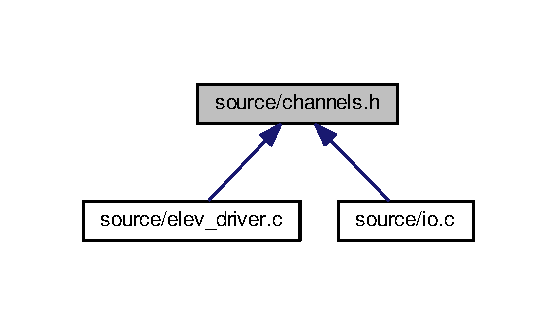
\includegraphics[width=268pt]{channels_8h__dep__incl}
\end{center}
\end{figure}
\subsection*{Macros}
\begin{DoxyCompactItemize}
\item 
\#define {\bfseries P\+O\+R\+T4}~3\hypertarget{channels_8h_ad5a54f368997d8ae4f84a1e2fad533f4}{}\label{channels_8h_ad5a54f368997d8ae4f84a1e2fad533f4}

\item 
\#define {\bfseries O\+B\+S\+T\+R\+U\+C\+T\+I\+ON}~(0x300+23)\hypertarget{channels_8h_a2409f02d98d288f64712887bd13b853e}{}\label{channels_8h_a2409f02d98d288f64712887bd13b853e}

\item 
\#define {\bfseries S\+T\+OP}~(0x300+22)\hypertarget{channels_8h_ae19b6bb2940d2fbe0a79852b070eeafd}{}\label{channels_8h_ae19b6bb2940d2fbe0a79852b070eeafd}

\item 
\#define {\bfseries B\+U\+T\+T\+O\+N\+\_\+\+C\+O\+M\+M\+A\+N\+D1}~(0x300+21)\hypertarget{channels_8h_a1a22e01173ae543c7350d23af9099083}{}\label{channels_8h_a1a22e01173ae543c7350d23af9099083}

\item 
\#define {\bfseries B\+U\+T\+T\+O\+N\+\_\+\+C\+O\+M\+M\+A\+N\+D2}~(0x300+20)\hypertarget{channels_8h_a8f3d02fddfb1ecd5227eca135f19ebd6}{}\label{channels_8h_a8f3d02fddfb1ecd5227eca135f19ebd6}

\item 
\#define {\bfseries B\+U\+T\+T\+O\+N\+\_\+\+C\+O\+M\+M\+A\+N\+D3}~(0x300+19)\hypertarget{channels_8h_a82aab21b1b50d554effcf8b26576b388}{}\label{channels_8h_a82aab21b1b50d554effcf8b26576b388}

\item 
\#define {\bfseries B\+U\+T\+T\+O\+N\+\_\+\+C\+O\+M\+M\+A\+N\+D4}~(0x300+18)\hypertarget{channels_8h_add9ae7df96dfd4ad569d3b703023187d}{}\label{channels_8h_add9ae7df96dfd4ad569d3b703023187d}

\item 
\#define {\bfseries B\+U\+T\+T\+O\+N\+\_\+\+U\+P1}~(0x300+17)\hypertarget{channels_8h_a7236f6ea90139248afabe014632c3cec}{}\label{channels_8h_a7236f6ea90139248afabe014632c3cec}

\item 
\#define {\bfseries B\+U\+T\+T\+O\+N\+\_\+\+U\+P2}~(0x300+16)\hypertarget{channels_8h_a3a95d31cf2002937c921bbd85590bc7a}{}\label{channels_8h_a3a95d31cf2002937c921bbd85590bc7a}

\item 
\#define {\bfseries P\+O\+R\+T1}~2\hypertarget{channels_8h_a83b698b796fa8d1625536439f28ea575}{}\label{channels_8h_a83b698b796fa8d1625536439f28ea575}

\item 
\#define {\bfseries B\+U\+T\+T\+O\+N\+\_\+\+D\+O\+W\+N2}~(0x200+0)\hypertarget{channels_8h_a63a7b9d9d7c23325d4171292d596fa11}{}\label{channels_8h_a63a7b9d9d7c23325d4171292d596fa11}

\item 
\#define {\bfseries B\+U\+T\+T\+O\+N\+\_\+\+U\+P3}~(0x200+1)\hypertarget{channels_8h_aa6b5917715e012cf21e3a89fb7c93e2d}{}\label{channels_8h_aa6b5917715e012cf21e3a89fb7c93e2d}

\item 
\#define {\bfseries B\+U\+T\+T\+O\+N\+\_\+\+D\+O\+W\+N3}~(0x200+2)\hypertarget{channels_8h_ab423174da71ed0d6b083cd8d71f54617}{}\label{channels_8h_ab423174da71ed0d6b083cd8d71f54617}

\item 
\#define {\bfseries B\+U\+T\+T\+O\+N\+\_\+\+D\+O\+W\+N4}~(0x200+3)\hypertarget{channels_8h_a7e1266fcb6843826718edec0222b1e49}{}\label{channels_8h_a7e1266fcb6843826718edec0222b1e49}

\item 
\#define {\bfseries S\+E\+N\+S\+O\+R\+\_\+\+F\+L\+O\+O\+R1}~(0x200+4)\hypertarget{channels_8h_a5ae95fe4e1273653467895d5e7c39377}{}\label{channels_8h_a5ae95fe4e1273653467895d5e7c39377}

\item 
\#define {\bfseries S\+E\+N\+S\+O\+R\+\_\+\+F\+L\+O\+O\+R2}~(0x200+5)\hypertarget{channels_8h_ab9e1c393bf2c51d65ed0a132af8321d3}{}\label{channels_8h_ab9e1c393bf2c51d65ed0a132af8321d3}

\item 
\#define {\bfseries S\+E\+N\+S\+O\+R\+\_\+\+F\+L\+O\+O\+R3}~(0x200+6)\hypertarget{channels_8h_a65904322d022513386fea3bcb9a8b524}{}\label{channels_8h_a65904322d022513386fea3bcb9a8b524}

\item 
\#define {\bfseries S\+E\+N\+S\+O\+R\+\_\+\+F\+L\+O\+O\+R4}~(0x200+7)\hypertarget{channels_8h_a6a8d30abdce8780479ac7f0677200074}{}\label{channels_8h_a6a8d30abdce8780479ac7f0677200074}

\item 
\#define {\bfseries P\+O\+R\+T3}~3\hypertarget{channels_8h_ad906b7f6a811f1f02b5eb04cbe1bc89b}{}\label{channels_8h_ad906b7f6a811f1f02b5eb04cbe1bc89b}

\item 
\#define {\bfseries M\+O\+T\+O\+R\+D\+IR}~(0x300+15)\hypertarget{channels_8h_aaa316c7fc13ca7b9b4229af3f9832a7d}{}\label{channels_8h_aaa316c7fc13ca7b9b4229af3f9832a7d}

\item 
\#define {\bfseries L\+I\+G\+H\+T\+\_\+\+S\+T\+OP}~(0x300+14)\hypertarget{channels_8h_a7845eb8e4ab5e0a49739663d69ff9001}{}\label{channels_8h_a7845eb8e4ab5e0a49739663d69ff9001}

\item 
\#define {\bfseries L\+I\+G\+H\+T\+\_\+\+C\+O\+M\+M\+A\+N\+D1}~(0x300+13)\hypertarget{channels_8h_a61e8bfbed9e1d63bbbce251b10b69d9b}{}\label{channels_8h_a61e8bfbed9e1d63bbbce251b10b69d9b}

\item 
\#define {\bfseries L\+I\+G\+H\+T\+\_\+\+C\+O\+M\+M\+A\+N\+D2}~(0x300+12)\hypertarget{channels_8h_a05423733c25f39ca059f5bfae9e3fb33}{}\label{channels_8h_a05423733c25f39ca059f5bfae9e3fb33}

\item 
\#define {\bfseries L\+I\+G\+H\+T\+\_\+\+C\+O\+M\+M\+A\+N\+D3}~(0x300+11)\hypertarget{channels_8h_aec8c2b567fd77cff4163ebab81b6abd1}{}\label{channels_8h_aec8c2b567fd77cff4163ebab81b6abd1}

\item 
\#define {\bfseries L\+I\+G\+H\+T\+\_\+\+C\+O\+M\+M\+A\+N\+D4}~(0x300+10)\hypertarget{channels_8h_ad2ffefe386fcbad6a538f84c7fe191f3}{}\label{channels_8h_ad2ffefe386fcbad6a538f84c7fe191f3}

\item 
\#define {\bfseries L\+I\+G\+H\+T\+\_\+\+U\+P1}~(0x300+9)\hypertarget{channels_8h_aec0494e52bb28dfa15a8035c3359bd0f}{}\label{channels_8h_aec0494e52bb28dfa15a8035c3359bd0f}

\item 
\#define {\bfseries L\+I\+G\+H\+T\+\_\+\+U\+P2}~(0x300+8)\hypertarget{channels_8h_ab4f192467448356764080a8102eb32f1}{}\label{channels_8h_ab4f192467448356764080a8102eb32f1}

\item 
\#define {\bfseries P\+O\+R\+T2}~3\hypertarget{channels_8h_acb270e4aec8a0ab123e6c24a5810150b}{}\label{channels_8h_acb270e4aec8a0ab123e6c24a5810150b}

\item 
\#define {\bfseries L\+I\+G\+H\+T\+\_\+\+D\+O\+W\+N2}~(0x300+7)\hypertarget{channels_8h_a919d92344f7934414150b99fe94d1ace}{}\label{channels_8h_a919d92344f7934414150b99fe94d1ace}

\item 
\#define {\bfseries L\+I\+G\+H\+T\+\_\+\+U\+P3}~(0x300+6)\hypertarget{channels_8h_a2fd78cafe153eb500f5f6731f6a2d7c7}{}\label{channels_8h_a2fd78cafe153eb500f5f6731f6a2d7c7}

\item 
\#define {\bfseries L\+I\+G\+H\+T\+\_\+\+D\+O\+W\+N3}~(0x300+5)\hypertarget{channels_8h_adc5182903fbf37402ed9a2b65af65a40}{}\label{channels_8h_adc5182903fbf37402ed9a2b65af65a40}

\item 
\#define {\bfseries L\+I\+G\+H\+T\+\_\+\+D\+O\+W\+N4}~(0x300+4)\hypertarget{channels_8h_a1745b9fd720072a9ff8f58c75ca9512c}{}\label{channels_8h_a1745b9fd720072a9ff8f58c75ca9512c}

\item 
\#define {\bfseries L\+I\+G\+H\+T\+\_\+\+D\+O\+O\+R\+\_\+\+O\+P\+EN}~(0x300+3)\hypertarget{channels_8h_ab3e81b38bff9c0c8dd9dea97f3c42073}{}\label{channels_8h_ab3e81b38bff9c0c8dd9dea97f3c42073}

\item 
\#define {\bfseries L\+I\+G\+H\+T\+\_\+\+F\+L\+O\+O\+R\+\_\+\+I\+N\+D2}~(0x300+1)\hypertarget{channels_8h_a99e7a2989cfe5f085c49c31d033baae2}{}\label{channels_8h_a99e7a2989cfe5f085c49c31d033baae2}

\item 
\#define {\bfseries L\+I\+G\+H\+T\+\_\+\+F\+L\+O\+O\+R\+\_\+\+I\+N\+D1}~(0x300+0)\hypertarget{channels_8h_a1b686be38adf6a919cceca00890df7c8}{}\label{channels_8h_a1b686be38adf6a919cceca00890df7c8}

\item 
\#define {\bfseries P\+O\+R\+T0}~1\hypertarget{channels_8h_af41b34488a518db05b413d3a370f871f}{}\label{channels_8h_af41b34488a518db05b413d3a370f871f}

\item 
\#define {\bfseries M\+O\+T\+OR}~(0x100+0)\hypertarget{channels_8h_ae8d3b23b31729f61bc738fbd9a9a24e0}{}\label{channels_8h_ae8d3b23b31729f61bc738fbd9a9a24e0}

\item 
\#define {\bfseries B\+U\+T\+T\+O\+N\+\_\+\+D\+O\+W\+N1}~-\/1\hypertarget{channels_8h_a8bcc98057f83b3b335fa3d9865410d42}{}\label{channels_8h_a8bcc98057f83b3b335fa3d9865410d42}

\item 
\#define {\bfseries B\+U\+T\+T\+O\+N\+\_\+\+U\+P4}~-\/1\hypertarget{channels_8h_a02cc4cce547c81453cf7b5e55dd24986}{}\label{channels_8h_a02cc4cce547c81453cf7b5e55dd24986}

\item 
\#define {\bfseries L\+I\+G\+H\+T\+\_\+\+D\+O\+W\+N1}~-\/1\hypertarget{channels_8h_ad63056bd0003fdef7bdf927bf2ff1118}{}\label{channels_8h_ad63056bd0003fdef7bdf927bf2ff1118}

\item 
\#define {\bfseries L\+I\+G\+H\+T\+\_\+\+U\+P4}~-\/1\hypertarget{channels_8h_ab4e1e3be316a23e33d3080931737eb60}{}\label{channels_8h_ab4e1e3be316a23e33d3080931737eb60}

\end{DoxyCompactItemize}


\subsection{Detailed Description}
Channel definitions for elevator control using Lib\+Comedi. 


\hypertarget{controller_8h}{}\section{source/controller.h File Reference}
\label{controller_8h}\index{source/controller.\+h@{source/controller.\+h}}


Functions for controlling state of elevator.  


{\ttfamily \#include \char`\"{}elev\+\_\+driver.\+h\char`\"{}}\\*
{\ttfamily \#include \char`\"{}state\+\_\+machine.\+h\char`\"{}}\\*
Include dependency graph for controller.\+h\+:
\nopagebreak
\begin{figure}[H]
\begin{center}
\leavevmode
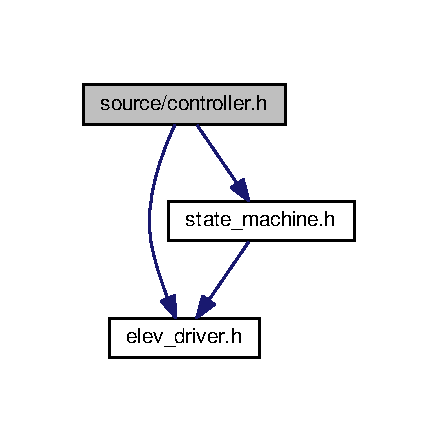
\includegraphics[width=210pt]{controller_8h__incl}
\end{center}
\end{figure}
This graph shows which files directly or indirectly include this file\+:\nopagebreak
\begin{figure}[H]
\begin{center}
\leavevmode
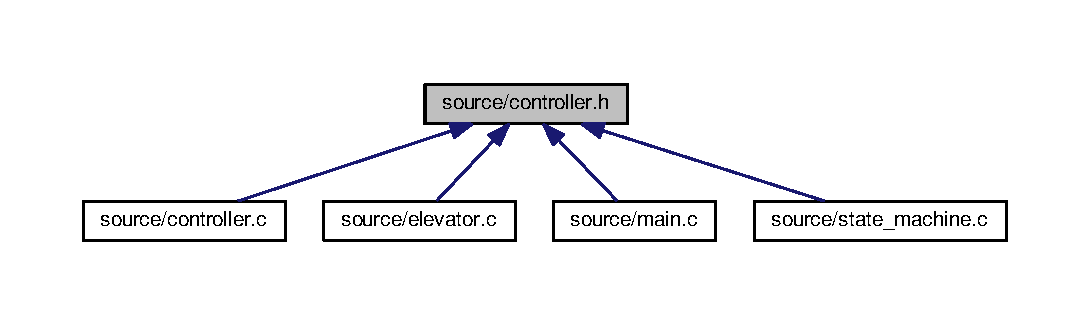
\includegraphics[width=350pt]{controller_8h__dep__incl}
\end{center}
\end{figure}
\subsection*{Functions}
\begin{DoxyCompactItemize}
\item 
state \hyperlink{controller_8h_a8e4d0ac3807643ff16f19831fec588e4}{next\+\_\+state} ()
\begin{DoxyCompactList}\small\item\em Finds the next state for the elevator. \end{DoxyCompactList}\item 
\hyperlink{elev__driver_8h_a2256dfd58fecce253106f83fd2ed607f}{elev\+\_\+motor\+\_\+direction\+\_\+t} \hyperlink{controller_8h_aeea5374cacd9bc0f1dd4579bd6cb0f46}{choose\+\_\+dir} ()
\begin{DoxyCompactList}\small\item\em Chooses which direction the elevator should drive next. \end{DoxyCompactList}\item 
void \hyperlink{controller_8h_a9a16f6b98f5f76be46fe27e82bba227b}{floor\+\_\+sensor\+\_\+poller} ()
\begin{DoxyCompactList}\small\item\em Checks floor sensor and sets the elevators current floor. If the elevator is at a floor, last floor is set and floor lights are updated. \end{DoxyCompactList}\item 
void \hyperlink{controller_8h_a57ae9c150db7661cef241d5e6001590f}{button\+\_\+poller} ()
\begin{DoxyCompactList}\small\item\em Checks if any buttons is pressed, and if so, adds the corresponding order to the orderlist. \end{DoxyCompactList}\item 
void \hyperlink{controller_8h_ac0fbceb0a5659d068173ed56670b5487}{update\+\_\+floor\+\_\+lights} (int last\+\_\+floor)
\begin{DoxyCompactList}\small\item\em Sets floor lights at . \end{DoxyCompactList}\end{DoxyCompactItemize}


\subsection{Detailed Description}
Functions for controlling state of elevator. 



\subsection{Function Documentation}
\index{controller.\+h@{controller.\+h}!button\+\_\+poller@{button\+\_\+poller}}
\index{button\+\_\+poller@{button\+\_\+poller}!controller.\+h@{controller.\+h}}
\subsubsection[{\texorpdfstring{button\+\_\+poller()}{button_poller()}}]{\setlength{\rightskip}{0pt plus 5cm}void button\+\_\+poller (
\begin{DoxyParamCaption}
{}
\end{DoxyParamCaption}
)}\hypertarget{controller_8h_a57ae9c150db7661cef241d5e6001590f}{}\label{controller_8h_a57ae9c150db7661cef241d5e6001590f}


Checks if any buttons is pressed, and if so, adds the corresponding order to the orderlist. 



Definition at line 69 of file controller.\+c.

\index{controller.\+h@{controller.\+h}!choose\+\_\+dir@{choose\+\_\+dir}}
\index{choose\+\_\+dir@{choose\+\_\+dir}!controller.\+h@{controller.\+h}}
\subsubsection[{\texorpdfstring{choose\+\_\+dir()}{choose_dir()}}]{\setlength{\rightskip}{0pt plus 5cm}{\bf elev\+\_\+motor\+\_\+direction\+\_\+t} choose\+\_\+dir (
\begin{DoxyParamCaption}
{}
\end{DoxyParamCaption}
)}\hypertarget{controller_8h_aeea5374cacd9bc0f1dd4579bd6cb0f46}{}\label{controller_8h_aeea5374cacd9bc0f1dd4579bd6cb0f46}


Chooses which direction the elevator should drive next. 

\begin{DoxyReturn}{Returns}
New direction for the elevator. 
\end{DoxyReturn}


Definition at line 25 of file controller.\+c.

\index{controller.\+h@{controller.\+h}!floor\+\_\+sensor\+\_\+poller@{floor\+\_\+sensor\+\_\+poller}}
\index{floor\+\_\+sensor\+\_\+poller@{floor\+\_\+sensor\+\_\+poller}!controller.\+h@{controller.\+h}}
\subsubsection[{\texorpdfstring{floor\+\_\+sensor\+\_\+poller()}{floor_sensor_poller()}}]{\setlength{\rightskip}{0pt plus 5cm}void floor\+\_\+sensor\+\_\+poller (
\begin{DoxyParamCaption}
{}
\end{DoxyParamCaption}
)}\hypertarget{controller_8h_a9a16f6b98f5f76be46fe27e82bba227b}{}\label{controller_8h_a9a16f6b98f5f76be46fe27e82bba227b}


Checks floor sensor and sets the elevators current floor. If the elevator is at a floor, last floor is set and floor lights are updated. 



Definition at line 60 of file controller.\+c.

\index{controller.\+h@{controller.\+h}!next\+\_\+state@{next\+\_\+state}}
\index{next\+\_\+state@{next\+\_\+state}!controller.\+h@{controller.\+h}}
\subsubsection[{\texorpdfstring{next\+\_\+state()}{next_state()}}]{\setlength{\rightskip}{0pt plus 5cm}state next\+\_\+state (
\begin{DoxyParamCaption}
{}
\end{DoxyParamCaption}
)}\hypertarget{controller_8h_a8e4d0ac3807643ff16f19831fec588e4}{}\label{controller_8h_a8e4d0ac3807643ff16f19831fec588e4}


Finds the next state for the elevator. 

\begin{DoxyReturn}{Returns}
Next state for the elevator. Returns -\/1 if no valid state. 
\end{DoxyReturn}


Definition at line 9 of file controller.\+c.

\index{controller.\+h@{controller.\+h}!update\+\_\+floor\+\_\+lights@{update\+\_\+floor\+\_\+lights}}
\index{update\+\_\+floor\+\_\+lights@{update\+\_\+floor\+\_\+lights}!controller.\+h@{controller.\+h}}
\subsubsection[{\texorpdfstring{update\+\_\+floor\+\_\+lights(int last\+\_\+floor)}{update_floor_lights(int last_floor)}}]{\setlength{\rightskip}{0pt plus 5cm}void update\+\_\+floor\+\_\+lights (
\begin{DoxyParamCaption}
\item[{int}]{last\+\_\+floor}
\end{DoxyParamCaption}
)}\hypertarget{controller_8h_ac0fbceb0a5659d068173ed56670b5487}{}\label{controller_8h_ac0fbceb0a5659d068173ed56670b5487}


Sets floor lights at . 


\begin{DoxyParams}[1]{Parameters}
\mbox{\tt in}  & {\em last\+\_\+floor} & The floor where the sensor was last indicated. \\
\hline
\end{DoxyParams}


Definition at line 82 of file controller.\+c.


\hypertarget{elev__driver_8c}{}\section{source/elev\+\_\+driver.c File Reference}
\label{elev__driver_8c}\index{source/elev\+\_\+driver.\+c@{source/elev\+\_\+driver.\+c}}
{\ttfamily \#include \char`\"{}channels.\+h\char`\"{}}\\*
{\ttfamily \#include \char`\"{}elev\+\_\+driver.\+h\char`\"{}}\\*
{\ttfamily \#include \char`\"{}io.\+h\char`\"{}}\\*
{\ttfamily \#include $<$assert.\+h$>$}\\*
{\ttfamily \#include $<$stdlib.\+h$>$}\\*
Include dependency graph for elev\+\_\+driver.\+c\+:
\nopagebreak
\begin{figure}[H]
\begin{center}
\leavevmode
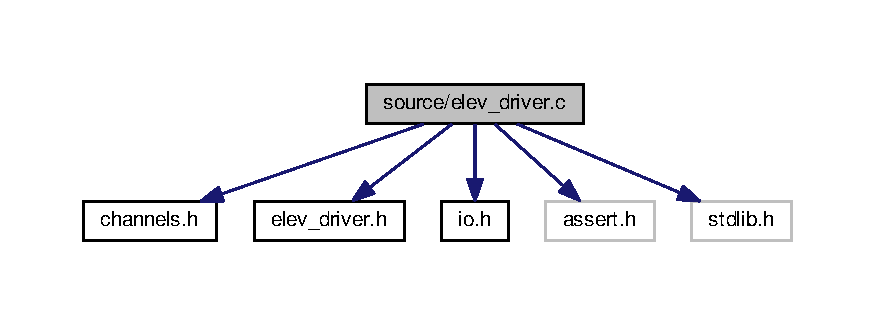
\includegraphics[width=350pt]{elev__driver_8c__incl}
\end{center}
\end{figure}
\subsection*{Functions}
\begin{DoxyCompactItemize}
\item 
int \hyperlink{elev__driver_8c_a949b0e1f7c0f03ea6f92008c378e4573}{elev\+\_\+init} (void)
\item 
void \hyperlink{elev__driver_8c_ac7dccb879f6e812e9d245174a0214536}{elev\+\_\+set\+\_\+motor\+\_\+direction} (\hyperlink{elev__driver_8h_a2256dfd58fecce253106f83fd2ed607f}{elev\+\_\+motor\+\_\+direction\+\_\+t} dirn)
\item 
void \hyperlink{elev__driver_8c_a6ce9a34b8677b483b0d8f9dc47b42c40}{elev\+\_\+set\+\_\+door\+\_\+open\+\_\+lamp} (int value)
\item 
int \hyperlink{elev__driver_8c_acd97a0fbc9013dc954923e25e90be9df}{elev\+\_\+get\+\_\+obstruction\+\_\+signal} (void)
\item 
int \hyperlink{elev__driver_8c_ab702d0ff2d7d03172b7ae3829ba13028}{elev\+\_\+get\+\_\+stop\+\_\+signal} (void)
\item 
void \hyperlink{elev__driver_8c_a85de2a6536b4dd0c83bac19923500740}{elev\+\_\+set\+\_\+stop\+\_\+lamp} (int value)
\item 
int \hyperlink{elev__driver_8c_a97d30b7e2538acf5647515638070fdc5}{elev\+\_\+get\+\_\+floor\+\_\+sensor\+\_\+signal} (void)
\item 
void \hyperlink{elev__driver_8c_a6af53dd3ebae3a5791ba345eac84d4be}{elev\+\_\+set\+\_\+floor\+\_\+indicator} (int floor)
\item 
int \hyperlink{elev__driver_8c_a2350a1635233760719700552a6cb0763}{elev\+\_\+get\+\_\+button\+\_\+signal} (\hyperlink{elev__driver_8h_af61c4136fb437a2c49037e5a57c9abda}{elev\+\_\+button\+\_\+type\+\_\+t} button, int floor)
\item 
void \hyperlink{elev__driver_8c_a9e81321c63d80ddf1699bc91593cd9d4}{elev\+\_\+set\+\_\+button\+\_\+lamp} (\hyperlink{elev__driver_8h_af61c4136fb437a2c49037e5a57c9abda}{elev\+\_\+button\+\_\+type\+\_\+t} button, int floor, int value)
\end{DoxyCompactItemize}


\subsection{Function Documentation}
\index{elev\+\_\+driver.\+c@{elev\+\_\+driver.\+c}!elev\+\_\+get\+\_\+button\+\_\+signal@{elev\+\_\+get\+\_\+button\+\_\+signal}}
\index{elev\+\_\+get\+\_\+button\+\_\+signal@{elev\+\_\+get\+\_\+button\+\_\+signal}!elev\+\_\+driver.\+c@{elev\+\_\+driver.\+c}}
\subsubsection[{\texorpdfstring{elev\+\_\+get\+\_\+button\+\_\+signal(elev\+\_\+button\+\_\+type\+\_\+t button, int floor)}{elev_get_button_signal(elev_button_type_t button, int floor)}}]{\setlength{\rightskip}{0pt plus 5cm}int elev\+\_\+get\+\_\+button\+\_\+signal (
\begin{DoxyParamCaption}
\item[{{\bf elev\+\_\+button\+\_\+type\+\_\+t}}]{button, }
\item[{int}]{floor}
\end{DoxyParamCaption}
)}\hypertarget{elev__driver_8c_a2350a1635233760719700552a6cb0763}{}\label{elev__driver_8c_a2350a1635233760719700552a6cb0763}
Gets a button signal. 
\begin{DoxyParams}{Parameters}
{\em button} & Which button type to check. Can be B\+U\+T\+T\+O\+N\+\_\+\+C\+A\+L\+L\+\_\+\+UP, B\+U\+T\+T\+O\+N\+\_\+\+C\+A\+L\+L\+\_\+\+D\+O\+WN or B\+U\+T\+T\+O\+N\+\_\+\+C\+O\+M\+M\+A\+ND (button "inside the elevator). \\
\hline
{\em floor} & Which floor to check button. Must be 0-\/3. \\
\hline
\end{DoxyParams}
\begin{DoxyReturn}{Returns}
0 if button is not pushed. 1 if button is pushed. 
\end{DoxyReturn}


Definition at line 123 of file elev\+\_\+driver.\+c.

\index{elev\+\_\+driver.\+c@{elev\+\_\+driver.\+c}!elev\+\_\+get\+\_\+floor\+\_\+sensor\+\_\+signal@{elev\+\_\+get\+\_\+floor\+\_\+sensor\+\_\+signal}}
\index{elev\+\_\+get\+\_\+floor\+\_\+sensor\+\_\+signal@{elev\+\_\+get\+\_\+floor\+\_\+sensor\+\_\+signal}!elev\+\_\+driver.\+c@{elev\+\_\+driver.\+c}}
\subsubsection[{\texorpdfstring{elev\+\_\+get\+\_\+floor\+\_\+sensor\+\_\+signal(void)}{elev_get_floor_sensor_signal(void)}}]{\setlength{\rightskip}{0pt plus 5cm}int elev\+\_\+get\+\_\+floor\+\_\+sensor\+\_\+signal (
\begin{DoxyParamCaption}
\item[{void}]{}
\end{DoxyParamCaption}
)}\hypertarget{elev__driver_8c_a97d30b7e2538acf5647515638070fdc5}{}\label{elev__driver_8c_a97d30b7e2538acf5647515638070fdc5}
Get floor sensor signal. \begin{DoxyReturn}{Returns}
-\/1 if elevator is not on a floor. 0-\/3 if elevator is on floor. 0 is ground floor, 3 is top floor. 
\end{DoxyReturn}


Definition at line 94 of file elev\+\_\+driver.\+c.

\index{elev\+\_\+driver.\+c@{elev\+\_\+driver.\+c}!elev\+\_\+get\+\_\+obstruction\+\_\+signal@{elev\+\_\+get\+\_\+obstruction\+\_\+signal}}
\index{elev\+\_\+get\+\_\+obstruction\+\_\+signal@{elev\+\_\+get\+\_\+obstruction\+\_\+signal}!elev\+\_\+driver.\+c@{elev\+\_\+driver.\+c}}
\subsubsection[{\texorpdfstring{elev\+\_\+get\+\_\+obstruction\+\_\+signal(void)}{elev_get_obstruction_signal(void)}}]{\setlength{\rightskip}{0pt plus 5cm}int elev\+\_\+get\+\_\+obstruction\+\_\+signal (
\begin{DoxyParamCaption}
\item[{void}]{}
\end{DoxyParamCaption}
)}\hypertarget{elev__driver_8c_acd97a0fbc9013dc954923e25e90be9df}{}\label{elev__driver_8c_acd97a0fbc9013dc954923e25e90be9df}
Get signal from obstruction switch. \begin{DoxyReturn}{Returns}
1 if obstruction is enabled. 0 if not. 
\end{DoxyReturn}


Definition at line 79 of file elev\+\_\+driver.\+c.

\index{elev\+\_\+driver.\+c@{elev\+\_\+driver.\+c}!elev\+\_\+get\+\_\+stop\+\_\+signal@{elev\+\_\+get\+\_\+stop\+\_\+signal}}
\index{elev\+\_\+get\+\_\+stop\+\_\+signal@{elev\+\_\+get\+\_\+stop\+\_\+signal}!elev\+\_\+driver.\+c@{elev\+\_\+driver.\+c}}
\subsubsection[{\texorpdfstring{elev\+\_\+get\+\_\+stop\+\_\+signal(void)}{elev_get_stop_signal(void)}}]{\setlength{\rightskip}{0pt plus 5cm}int elev\+\_\+get\+\_\+stop\+\_\+signal (
\begin{DoxyParamCaption}
\item[{void}]{}
\end{DoxyParamCaption}
)}\hypertarget{elev__driver_8c_ab702d0ff2d7d03172b7ae3829ba13028}{}\label{elev__driver_8c_ab702d0ff2d7d03172b7ae3829ba13028}
Get signal from stop button. \begin{DoxyReturn}{Returns}
1 if stop button is pushed, 0 if not. 
\end{DoxyReturn}


Definition at line 83 of file elev\+\_\+driver.\+c.

\index{elev\+\_\+driver.\+c@{elev\+\_\+driver.\+c}!elev\+\_\+init@{elev\+\_\+init}}
\index{elev\+\_\+init@{elev\+\_\+init}!elev\+\_\+driver.\+c@{elev\+\_\+driver.\+c}}
\subsubsection[{\texorpdfstring{elev\+\_\+init(void)}{elev_init(void)}}]{\setlength{\rightskip}{0pt plus 5cm}int elev\+\_\+init (
\begin{DoxyParamCaption}
\item[{void}]{}
\end{DoxyParamCaption}
)}\hypertarget{elev__driver_8c_a949b0e1f7c0f03ea6f92008c378e4573}{}\label{elev__driver_8c_a949b0e1f7c0f03ea6f92008c378e4573}
Initialize elevator. \begin{DoxyReturn}{Returns}
Non-\/zero on success, 0 on failure. 
\end{DoxyReturn}


Definition at line 33 of file elev\+\_\+driver.\+c.

\index{elev\+\_\+driver.\+c@{elev\+\_\+driver.\+c}!elev\+\_\+set\+\_\+button\+\_\+lamp@{elev\+\_\+set\+\_\+button\+\_\+lamp}}
\index{elev\+\_\+set\+\_\+button\+\_\+lamp@{elev\+\_\+set\+\_\+button\+\_\+lamp}!elev\+\_\+driver.\+c@{elev\+\_\+driver.\+c}}
\subsubsection[{\texorpdfstring{elev\+\_\+set\+\_\+button\+\_\+lamp(elev\+\_\+button\+\_\+type\+\_\+t button, int floor, int value)}{elev_set_button_lamp(elev_button_type_t button, int floor, int value)}}]{\setlength{\rightskip}{0pt plus 5cm}void elev\+\_\+set\+\_\+button\+\_\+lamp (
\begin{DoxyParamCaption}
\item[{{\bf elev\+\_\+button\+\_\+type\+\_\+t}}]{button, }
\item[{int}]{floor, }
\item[{int}]{value}
\end{DoxyParamCaption}
)}\hypertarget{elev__driver_8c_a9e81321c63d80ddf1699bc91593cd9d4}{}\label{elev__driver_8c_a9e81321c63d80ddf1699bc91593cd9d4}
Set a button lamp. 
\begin{DoxyParams}{Parameters}
{\em lamp} & Which type of lamp to set. Can be B\+U\+T\+T\+O\+N\+\_\+\+C\+A\+L\+L\+\_\+\+UP, B\+U\+T\+T\+O\+N\+\_\+\+C\+A\+L\+L\+\_\+\+D\+O\+WN or B\+U\+T\+T\+O\+N\+\_\+\+C\+O\+M\+M\+A\+ND (button \char`\"{}inside\char`\"{} the elevator). \\
\hline
{\em floor} & Floor of lamp to set. Must be 0-\/3 \\
\hline
{\em value} & Non-\/zero value turns lamp on, 0 turns lamp off. \\
\hline
\end{DoxyParams}


Definition at line 136 of file elev\+\_\+driver.\+c.

\index{elev\+\_\+driver.\+c@{elev\+\_\+driver.\+c}!elev\+\_\+set\+\_\+door\+\_\+open\+\_\+lamp@{elev\+\_\+set\+\_\+door\+\_\+open\+\_\+lamp}}
\index{elev\+\_\+set\+\_\+door\+\_\+open\+\_\+lamp@{elev\+\_\+set\+\_\+door\+\_\+open\+\_\+lamp}!elev\+\_\+driver.\+c@{elev\+\_\+driver.\+c}}
\subsubsection[{\texorpdfstring{elev\+\_\+set\+\_\+door\+\_\+open\+\_\+lamp(int value)}{elev_set_door_open_lamp(int value)}}]{\setlength{\rightskip}{0pt plus 5cm}void elev\+\_\+set\+\_\+door\+\_\+open\+\_\+lamp (
\begin{DoxyParamCaption}
\item[{int}]{value}
\end{DoxyParamCaption}
)}\hypertarget{elev__driver_8c_a6ce9a34b8677b483b0d8f9dc47b42c40}{}\label{elev__driver_8c_a6ce9a34b8677b483b0d8f9dc47b42c40}
Turn door-\/open lamp on or off. 
\begin{DoxyParams}{Parameters}
{\em value} & Non-\/zero value turns lamp on, 0 turns lamp off. \\
\hline
\end{DoxyParams}


Definition at line 72 of file elev\+\_\+driver.\+c.

\index{elev\+\_\+driver.\+c@{elev\+\_\+driver.\+c}!elev\+\_\+set\+\_\+floor\+\_\+indicator@{elev\+\_\+set\+\_\+floor\+\_\+indicator}}
\index{elev\+\_\+set\+\_\+floor\+\_\+indicator@{elev\+\_\+set\+\_\+floor\+\_\+indicator}!elev\+\_\+driver.\+c@{elev\+\_\+driver.\+c}}
\subsubsection[{\texorpdfstring{elev\+\_\+set\+\_\+floor\+\_\+indicator(int floor)}{elev_set_floor_indicator(int floor)}}]{\setlength{\rightskip}{0pt plus 5cm}void elev\+\_\+set\+\_\+floor\+\_\+indicator (
\begin{DoxyParamCaption}
\item[{int}]{floor}
\end{DoxyParamCaption}
)}\hypertarget{elev__driver_8c_a6af53dd3ebae3a5791ba345eac84d4be}{}\label{elev__driver_8c_a6af53dd3ebae3a5791ba345eac84d4be}
Set floor indicator lamp for a given floor. 
\begin{DoxyParams}{Parameters}
{\em floor} & Which floor lamp to turn on. Other floor lamps are turned off. \\
\hline
\end{DoxyParams}


Definition at line 107 of file elev\+\_\+driver.\+c.

\index{elev\+\_\+driver.\+c@{elev\+\_\+driver.\+c}!elev\+\_\+set\+\_\+motor\+\_\+direction@{elev\+\_\+set\+\_\+motor\+\_\+direction}}
\index{elev\+\_\+set\+\_\+motor\+\_\+direction@{elev\+\_\+set\+\_\+motor\+\_\+direction}!elev\+\_\+driver.\+c@{elev\+\_\+driver.\+c}}
\subsubsection[{\texorpdfstring{elev\+\_\+set\+\_\+motor\+\_\+direction(elev\+\_\+motor\+\_\+direction\+\_\+t dirn)}{elev_set_motor_direction(elev_motor_direction_t dirn)}}]{\setlength{\rightskip}{0pt plus 5cm}void elev\+\_\+set\+\_\+motor\+\_\+direction (
\begin{DoxyParamCaption}
\item[{{\bf elev\+\_\+motor\+\_\+direction\+\_\+t}}]{dirn}
\end{DoxyParamCaption}
)}\hypertarget{elev__driver_8c_ac7dccb879f6e812e9d245174a0214536}{}\label{elev__driver_8c_ac7dccb879f6e812e9d245174a0214536}
Sets the motor direction of the elevator. 
\begin{DoxyParams}{Parameters}
{\em dirn} & New direction of the elevator. \\
\hline
\end{DoxyParams}


Definition at line 60 of file elev\+\_\+driver.\+c.

\index{elev\+\_\+driver.\+c@{elev\+\_\+driver.\+c}!elev\+\_\+set\+\_\+stop\+\_\+lamp@{elev\+\_\+set\+\_\+stop\+\_\+lamp}}
\index{elev\+\_\+set\+\_\+stop\+\_\+lamp@{elev\+\_\+set\+\_\+stop\+\_\+lamp}!elev\+\_\+driver.\+c@{elev\+\_\+driver.\+c}}
\subsubsection[{\texorpdfstring{elev\+\_\+set\+\_\+stop\+\_\+lamp(int value)}{elev_set_stop_lamp(int value)}}]{\setlength{\rightskip}{0pt plus 5cm}void elev\+\_\+set\+\_\+stop\+\_\+lamp (
\begin{DoxyParamCaption}
\item[{int}]{value}
\end{DoxyParamCaption}
)}\hypertarget{elev__driver_8c_a85de2a6536b4dd0c83bac19923500740}{}\label{elev__driver_8c_a85de2a6536b4dd0c83bac19923500740}
Turn stop lamp on or off. 
\begin{DoxyParams}{Parameters}
{\em value} & Non-\/zero value turns lamp on, 0 turns lamp off. \\
\hline
\end{DoxyParams}


Definition at line 87 of file elev\+\_\+driver.\+c.


\hypertarget{elev__driver_8h}{}\section{source/elev\+\_\+driver.h File Reference}
\label{elev__driver_8h}\index{source/elev\+\_\+driver.\+h@{source/elev\+\_\+driver.\+h}}


Functions that provide an interface to the elevators in the real time lab.  


This graph shows which files directly or indirectly include this file\+:
\nopagebreak
\begin{figure}[H]
\begin{center}
\leavevmode
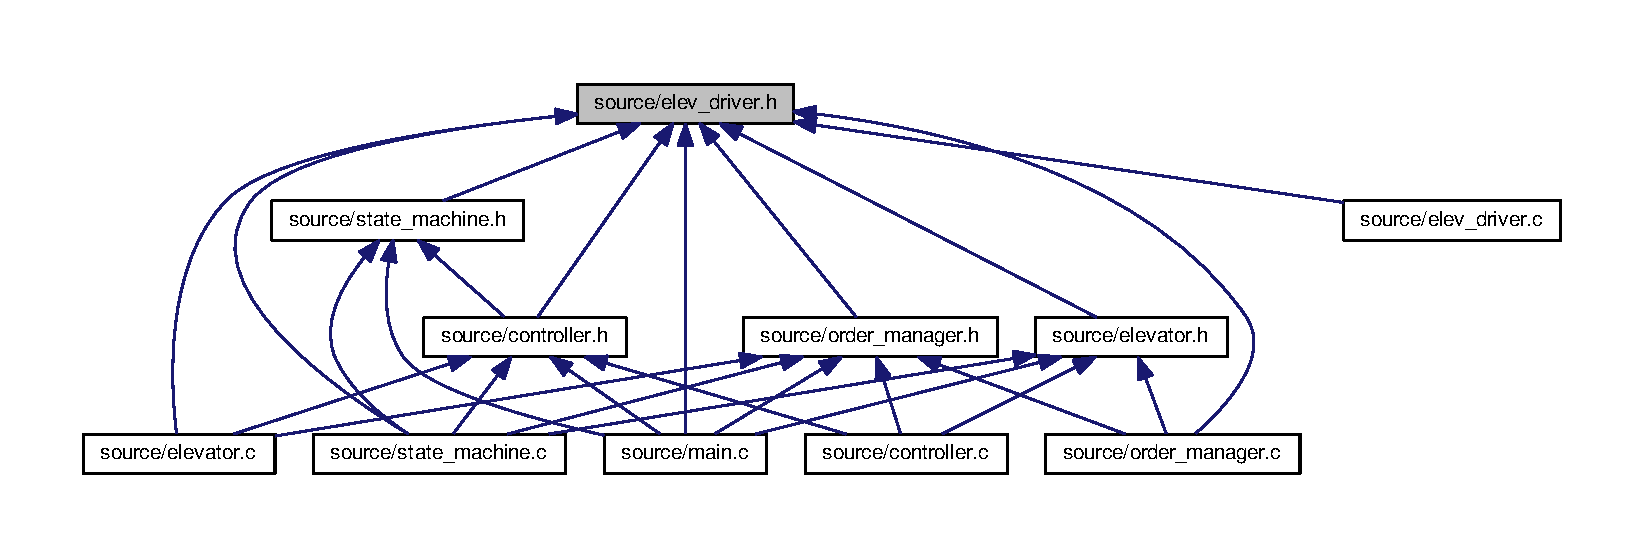
\includegraphics[width=350pt]{elev__driver_8h__dep__incl}
\end{center}
\end{figure}
\subsection*{Macros}
\begin{DoxyCompactItemize}
\item 
\#define {\bfseries N\+\_\+\+F\+L\+O\+O\+RS}~4\hypertarget{elev__driver_8h_ae0592e3739e5e1e76234bb1caf9d1305}{}\label{elev__driver_8h_ae0592e3739e5e1e76234bb1caf9d1305}

\item 
\#define {\bfseries N\+\_\+\+B\+U\+T\+T\+O\+NS}~3\hypertarget{elev__driver_8h_a271dda243b0f5bd7d2053d258eb71962}{}\label{elev__driver_8h_a271dda243b0f5bd7d2053d258eb71962}

\end{DoxyCompactItemize}
\subsection*{Typedefs}
\begin{DoxyCompactItemize}
\item 
typedef enum \hyperlink{elev__driver_8h_aaf85d173ea1bbd3d99c5a2fcf58cba11}{tag\+\_\+elev\+\_\+motor\+\_\+direction} \hyperlink{elev__driver_8h_a2256dfd58fecce253106f83fd2ed607f}{elev\+\_\+motor\+\_\+direction\+\_\+t}
\item 
typedef enum \hyperlink{elev__driver_8h_a0c3f8374e6ebcc71f91341eb3ba6f6f9}{tag\+\_\+elev\+\_\+lamp\+\_\+type} \hyperlink{elev__driver_8h_af61c4136fb437a2c49037e5a57c9abda}{elev\+\_\+button\+\_\+type\+\_\+t}
\end{DoxyCompactItemize}
\subsection*{Enumerations}
\begin{DoxyCompactItemize}
\item 
enum \hyperlink{elev__driver_8h_aaf85d173ea1bbd3d99c5a2fcf58cba11}{tag\+\_\+elev\+\_\+motor\+\_\+direction} \{ {\bfseries D\+I\+R\+N\+\_\+\+D\+O\+WN} = -\/1, 
{\bfseries D\+I\+R\+N\+\_\+\+S\+T\+OP} = 0, 
{\bfseries D\+I\+R\+N\+\_\+\+UP} = 1
 \}
\item 
enum \hyperlink{elev__driver_8h_a0c3f8374e6ebcc71f91341eb3ba6f6f9}{tag\+\_\+elev\+\_\+lamp\+\_\+type} \{ {\bfseries B\+U\+T\+T\+O\+N\+\_\+\+C\+A\+L\+L\+\_\+\+UP} = 0, 
{\bfseries B\+U\+T\+T\+O\+N\+\_\+\+C\+A\+L\+L\+\_\+\+D\+O\+WN} = 1, 
{\bfseries B\+U\+T\+T\+O\+N\+\_\+\+C\+O\+M\+M\+A\+ND} = 2
 \}
\end{DoxyCompactItemize}
\subsection*{Functions}
\begin{DoxyCompactItemize}
\item 
int \hyperlink{elev__driver_8h_a949b0e1f7c0f03ea6f92008c378e4573}{elev\+\_\+init} (void)
\item 
void \hyperlink{elev__driver_8h_ac7dccb879f6e812e9d245174a0214536}{elev\+\_\+set\+\_\+motor\+\_\+direction} (\hyperlink{elev__driver_8h_a2256dfd58fecce253106f83fd2ed607f}{elev\+\_\+motor\+\_\+direction\+\_\+t} dirn)
\item 
void \hyperlink{elev__driver_8h_a6ce9a34b8677b483b0d8f9dc47b42c40}{elev\+\_\+set\+\_\+door\+\_\+open\+\_\+lamp} (int value)
\item 
int \hyperlink{elev__driver_8h_acd97a0fbc9013dc954923e25e90be9df}{elev\+\_\+get\+\_\+obstruction\+\_\+signal} (void)
\item 
int \hyperlink{elev__driver_8h_ab702d0ff2d7d03172b7ae3829ba13028}{elev\+\_\+get\+\_\+stop\+\_\+signal} (void)
\item 
void \hyperlink{elev__driver_8h_a85de2a6536b4dd0c83bac19923500740}{elev\+\_\+set\+\_\+stop\+\_\+lamp} (int value)
\item 
int \hyperlink{elev__driver_8h_a97d30b7e2538acf5647515638070fdc5}{elev\+\_\+get\+\_\+floor\+\_\+sensor\+\_\+signal} (void)
\item 
void \hyperlink{elev__driver_8h_a6af53dd3ebae3a5791ba345eac84d4be}{elev\+\_\+set\+\_\+floor\+\_\+indicator} (int floor)
\item 
int \hyperlink{elev__driver_8h_a2350a1635233760719700552a6cb0763}{elev\+\_\+get\+\_\+button\+\_\+signal} (\hyperlink{elev__driver_8h_af61c4136fb437a2c49037e5a57c9abda}{elev\+\_\+button\+\_\+type\+\_\+t} button, int floor)
\item 
void \hyperlink{elev__driver_8h_a9e81321c63d80ddf1699bc91593cd9d4}{elev\+\_\+set\+\_\+button\+\_\+lamp} (\hyperlink{elev__driver_8h_af61c4136fb437a2c49037e5a57c9abda}{elev\+\_\+button\+\_\+type\+\_\+t} button, int floor, int value)
\end{DoxyCompactItemize}


\subsection{Detailed Description}
Functions that provide an interface to the elevators in the real time lab. 



\subsection{Typedef Documentation}
\index{elev\+\_\+driver.\+h@{elev\+\_\+driver.\+h}!elev\+\_\+button\+\_\+type\+\_\+t@{elev\+\_\+button\+\_\+type\+\_\+t}}
\index{elev\+\_\+button\+\_\+type\+\_\+t@{elev\+\_\+button\+\_\+type\+\_\+t}!elev\+\_\+driver.\+h@{elev\+\_\+driver.\+h}}
\subsubsection[{\texorpdfstring{elev\+\_\+button\+\_\+type\+\_\+t}{elev_button_type_t}}]{\setlength{\rightskip}{0pt plus 5cm}typedef enum {\bf tag\+\_\+elev\+\_\+lamp\+\_\+type}  {\bf elev\+\_\+button\+\_\+type\+\_\+t}}\hypertarget{elev__driver_8h_af61c4136fb437a2c49037e5a57c9abda}{}\label{elev__driver_8h_af61c4136fb437a2c49037e5a57c9abda}
Button types for function \hyperlink{elev__driver_8c_a9e81321c63d80ddf1699bc91593cd9d4}{elev\+\_\+set\+\_\+button\+\_\+lamp()} and elev\+\_\+get\+\_\+button(). \index{elev\+\_\+driver.\+h@{elev\+\_\+driver.\+h}!elev\+\_\+motor\+\_\+direction\+\_\+t@{elev\+\_\+motor\+\_\+direction\+\_\+t}}
\index{elev\+\_\+motor\+\_\+direction\+\_\+t@{elev\+\_\+motor\+\_\+direction\+\_\+t}!elev\+\_\+driver.\+h@{elev\+\_\+driver.\+h}}
\subsubsection[{\texorpdfstring{elev\+\_\+motor\+\_\+direction\+\_\+t}{elev_motor_direction_t}}]{\setlength{\rightskip}{0pt plus 5cm}typedef enum {\bf tag\+\_\+elev\+\_\+motor\+\_\+direction}  {\bf elev\+\_\+motor\+\_\+direction\+\_\+t}}\hypertarget{elev__driver_8h_a2256dfd58fecce253106f83fd2ed607f}{}\label{elev__driver_8h_a2256dfd58fecce253106f83fd2ed607f}
Motor direction for function \hyperlink{elev__driver_8c_ac7dccb879f6e812e9d245174a0214536}{elev\+\_\+set\+\_\+motor\+\_\+direction()}. 

\subsection{Enumeration Type Documentation}
\index{elev\+\_\+driver.\+h@{elev\+\_\+driver.\+h}!tag\+\_\+elev\+\_\+lamp\+\_\+type@{tag\+\_\+elev\+\_\+lamp\+\_\+type}}
\index{tag\+\_\+elev\+\_\+lamp\+\_\+type@{tag\+\_\+elev\+\_\+lamp\+\_\+type}!elev\+\_\+driver.\+h@{elev\+\_\+driver.\+h}}
\subsubsection[{\texorpdfstring{tag\+\_\+elev\+\_\+lamp\+\_\+type}{tag_elev_lamp_type}}]{\setlength{\rightskip}{0pt plus 5cm}enum {\bf tag\+\_\+elev\+\_\+lamp\+\_\+type}}\hypertarget{elev__driver_8h_a0c3f8374e6ebcc71f91341eb3ba6f6f9}{}\label{elev__driver_8h_a0c3f8374e6ebcc71f91341eb3ba6f6f9}
Button types for function \hyperlink{elev__driver_8h_a9e81321c63d80ddf1699bc91593cd9d4}{elev\+\_\+set\+\_\+button\+\_\+lamp()} and elev\+\_\+get\+\_\+button(). 

Definition at line 98 of file elev\+\_\+driver.\+h.

\index{elev\+\_\+driver.\+h@{elev\+\_\+driver.\+h}!tag\+\_\+elev\+\_\+motor\+\_\+direction@{tag\+\_\+elev\+\_\+motor\+\_\+direction}}
\index{tag\+\_\+elev\+\_\+motor\+\_\+direction@{tag\+\_\+elev\+\_\+motor\+\_\+direction}!elev\+\_\+driver.\+h@{elev\+\_\+driver.\+h}}
\subsubsection[{\texorpdfstring{tag\+\_\+elev\+\_\+motor\+\_\+direction}{tag_elev_motor_direction}}]{\setlength{\rightskip}{0pt plus 5cm}enum {\bf tag\+\_\+elev\+\_\+motor\+\_\+direction}}\hypertarget{elev__driver_8h_aaf85d173ea1bbd3d99c5a2fcf58cba11}{}\label{elev__driver_8h_aaf85d173ea1bbd3d99c5a2fcf58cba11}
Motor direction for function \hyperlink{elev__driver_8h_ac7dccb879f6e812e9d245174a0214536}{elev\+\_\+set\+\_\+motor\+\_\+direction()}. 

Definition at line 30 of file elev\+\_\+driver.\+h.



\subsection{Function Documentation}
\index{elev\+\_\+driver.\+h@{elev\+\_\+driver.\+h}!elev\+\_\+get\+\_\+button\+\_\+signal@{elev\+\_\+get\+\_\+button\+\_\+signal}}
\index{elev\+\_\+get\+\_\+button\+\_\+signal@{elev\+\_\+get\+\_\+button\+\_\+signal}!elev\+\_\+driver.\+h@{elev\+\_\+driver.\+h}}
\subsubsection[{\texorpdfstring{elev\+\_\+get\+\_\+button\+\_\+signal(elev\+\_\+button\+\_\+type\+\_\+t button, int floor)}{elev_get_button_signal(elev_button_type_t button, int floor)}}]{\setlength{\rightskip}{0pt plus 5cm}int elev\+\_\+get\+\_\+button\+\_\+signal (
\begin{DoxyParamCaption}
\item[{{\bf elev\+\_\+button\+\_\+type\+\_\+t}}]{button, }
\item[{int}]{floor}
\end{DoxyParamCaption}
)}\hypertarget{elev__driver_8h_a2350a1635233760719700552a6cb0763}{}\label{elev__driver_8h_a2350a1635233760719700552a6cb0763}
Gets a button signal. 
\begin{DoxyParams}{Parameters}
{\em button} & Which button type to check. Can be B\+U\+T\+T\+O\+N\+\_\+\+C\+A\+L\+L\+\_\+\+UP, B\+U\+T\+T\+O\+N\+\_\+\+C\+A\+L\+L\+\_\+\+D\+O\+WN or B\+U\+T\+T\+O\+N\+\_\+\+C\+O\+M\+M\+A\+ND (button "inside the elevator). \\
\hline
{\em floor} & Which floor to check button. Must be 0-\/3. \\
\hline
\end{DoxyParams}
\begin{DoxyReturn}{Returns}
0 if button is not pushed. 1 if button is pushed. 
\end{DoxyReturn}


Definition at line 124 of file elev\+\_\+driver.\+c.

\index{elev\+\_\+driver.\+h@{elev\+\_\+driver.\+h}!elev\+\_\+get\+\_\+floor\+\_\+sensor\+\_\+signal@{elev\+\_\+get\+\_\+floor\+\_\+sensor\+\_\+signal}}
\index{elev\+\_\+get\+\_\+floor\+\_\+sensor\+\_\+signal@{elev\+\_\+get\+\_\+floor\+\_\+sensor\+\_\+signal}!elev\+\_\+driver.\+h@{elev\+\_\+driver.\+h}}
\subsubsection[{\texorpdfstring{elev\+\_\+get\+\_\+floor\+\_\+sensor\+\_\+signal(void)}{elev_get_floor_sensor_signal(void)}}]{\setlength{\rightskip}{0pt plus 5cm}int elev\+\_\+get\+\_\+floor\+\_\+sensor\+\_\+signal (
\begin{DoxyParamCaption}
\item[{void}]{}
\end{DoxyParamCaption}
)}\hypertarget{elev__driver_8h_a97d30b7e2538acf5647515638070fdc5}{}\label{elev__driver_8h_a97d30b7e2538acf5647515638070fdc5}
Get floor sensor signal. \begin{DoxyReturn}{Returns}
-\/1 if elevator is not on a floor. 0-\/3 if elevator is on floor. 0 is ground floor, 3 is top floor. 
\end{DoxyReturn}


Definition at line 95 of file elev\+\_\+driver.\+c.

\index{elev\+\_\+driver.\+h@{elev\+\_\+driver.\+h}!elev\+\_\+get\+\_\+obstruction\+\_\+signal@{elev\+\_\+get\+\_\+obstruction\+\_\+signal}}
\index{elev\+\_\+get\+\_\+obstruction\+\_\+signal@{elev\+\_\+get\+\_\+obstruction\+\_\+signal}!elev\+\_\+driver.\+h@{elev\+\_\+driver.\+h}}
\subsubsection[{\texorpdfstring{elev\+\_\+get\+\_\+obstruction\+\_\+signal(void)}{elev_get_obstruction_signal(void)}}]{\setlength{\rightskip}{0pt plus 5cm}int elev\+\_\+get\+\_\+obstruction\+\_\+signal (
\begin{DoxyParamCaption}
\item[{void}]{}
\end{DoxyParamCaption}
)}\hypertarget{elev__driver_8h_acd97a0fbc9013dc954923e25e90be9df}{}\label{elev__driver_8h_acd97a0fbc9013dc954923e25e90be9df}
Get signal from obstruction switch. \begin{DoxyReturn}{Returns}
1 if obstruction is enabled. 0 if not. 
\end{DoxyReturn}


Definition at line 80 of file elev\+\_\+driver.\+c.

\index{elev\+\_\+driver.\+h@{elev\+\_\+driver.\+h}!elev\+\_\+get\+\_\+stop\+\_\+signal@{elev\+\_\+get\+\_\+stop\+\_\+signal}}
\index{elev\+\_\+get\+\_\+stop\+\_\+signal@{elev\+\_\+get\+\_\+stop\+\_\+signal}!elev\+\_\+driver.\+h@{elev\+\_\+driver.\+h}}
\subsubsection[{\texorpdfstring{elev\+\_\+get\+\_\+stop\+\_\+signal(void)}{elev_get_stop_signal(void)}}]{\setlength{\rightskip}{0pt plus 5cm}int elev\+\_\+get\+\_\+stop\+\_\+signal (
\begin{DoxyParamCaption}
\item[{void}]{}
\end{DoxyParamCaption}
)}\hypertarget{elev__driver_8h_ab702d0ff2d7d03172b7ae3829ba13028}{}\label{elev__driver_8h_ab702d0ff2d7d03172b7ae3829ba13028}
Get signal from stop button. \begin{DoxyReturn}{Returns}
1 if stop button is pushed, 0 if not. 
\end{DoxyReturn}


Definition at line 84 of file elev\+\_\+driver.\+c.

\index{elev\+\_\+driver.\+h@{elev\+\_\+driver.\+h}!elev\+\_\+init@{elev\+\_\+init}}
\index{elev\+\_\+init@{elev\+\_\+init}!elev\+\_\+driver.\+h@{elev\+\_\+driver.\+h}}
\subsubsection[{\texorpdfstring{elev\+\_\+init(void)}{elev_init(void)}}]{\setlength{\rightskip}{0pt plus 5cm}int elev\+\_\+init (
\begin{DoxyParamCaption}
\item[{void}]{}
\end{DoxyParamCaption}
)}\hypertarget{elev__driver_8h_a949b0e1f7c0f03ea6f92008c378e4573}{}\label{elev__driver_8h_a949b0e1f7c0f03ea6f92008c378e4573}
Initialize elevator. \begin{DoxyReturn}{Returns}
Non-\/zero on success, 0 on failure. 
\end{DoxyReturn}


Definition at line 34 of file elev\+\_\+driver.\+c.

\index{elev\+\_\+driver.\+h@{elev\+\_\+driver.\+h}!elev\+\_\+set\+\_\+button\+\_\+lamp@{elev\+\_\+set\+\_\+button\+\_\+lamp}}
\index{elev\+\_\+set\+\_\+button\+\_\+lamp@{elev\+\_\+set\+\_\+button\+\_\+lamp}!elev\+\_\+driver.\+h@{elev\+\_\+driver.\+h}}
\subsubsection[{\texorpdfstring{elev\+\_\+set\+\_\+button\+\_\+lamp(elev\+\_\+button\+\_\+type\+\_\+t button, int floor, int value)}{elev_set_button_lamp(elev_button_type_t button, int floor, int value)}}]{\setlength{\rightskip}{0pt plus 5cm}void elev\+\_\+set\+\_\+button\+\_\+lamp (
\begin{DoxyParamCaption}
\item[{{\bf elev\+\_\+button\+\_\+type\+\_\+t}}]{button, }
\item[{int}]{floor, }
\item[{int}]{value}
\end{DoxyParamCaption}
)}\hypertarget{elev__driver_8h_a9e81321c63d80ddf1699bc91593cd9d4}{}\label{elev__driver_8h_a9e81321c63d80ddf1699bc91593cd9d4}
Set a button lamp. 
\begin{DoxyParams}{Parameters}
{\em lamp} & Which type of lamp to set. Can be B\+U\+T\+T\+O\+N\+\_\+\+C\+A\+L\+L\+\_\+\+UP, B\+U\+T\+T\+O\+N\+\_\+\+C\+A\+L\+L\+\_\+\+D\+O\+WN or B\+U\+T\+T\+O\+N\+\_\+\+C\+O\+M\+M\+A\+ND (button \char`\"{}inside\char`\"{} the elevator). \\
\hline
{\em floor} & Floor of lamp to set. Must be 0-\/3 \\
\hline
{\em value} & Non-\/zero value turns lamp on, 0 turns lamp off. \\
\hline
\end{DoxyParams}


Definition at line 137 of file elev\+\_\+driver.\+c.

\index{elev\+\_\+driver.\+h@{elev\+\_\+driver.\+h}!elev\+\_\+set\+\_\+door\+\_\+open\+\_\+lamp@{elev\+\_\+set\+\_\+door\+\_\+open\+\_\+lamp}}
\index{elev\+\_\+set\+\_\+door\+\_\+open\+\_\+lamp@{elev\+\_\+set\+\_\+door\+\_\+open\+\_\+lamp}!elev\+\_\+driver.\+h@{elev\+\_\+driver.\+h}}
\subsubsection[{\texorpdfstring{elev\+\_\+set\+\_\+door\+\_\+open\+\_\+lamp(int value)}{elev_set_door_open_lamp(int value)}}]{\setlength{\rightskip}{0pt plus 5cm}void elev\+\_\+set\+\_\+door\+\_\+open\+\_\+lamp (
\begin{DoxyParamCaption}
\item[{int}]{value}
\end{DoxyParamCaption}
)}\hypertarget{elev__driver_8h_a6ce9a34b8677b483b0d8f9dc47b42c40}{}\label{elev__driver_8h_a6ce9a34b8677b483b0d8f9dc47b42c40}
Turn door-\/open lamp on or off. 
\begin{DoxyParams}{Parameters}
{\em value} & Non-\/zero value turns lamp on, 0 turns lamp off. \\
\hline
\end{DoxyParams}


Definition at line 73 of file elev\+\_\+driver.\+c.

\index{elev\+\_\+driver.\+h@{elev\+\_\+driver.\+h}!elev\+\_\+set\+\_\+floor\+\_\+indicator@{elev\+\_\+set\+\_\+floor\+\_\+indicator}}
\index{elev\+\_\+set\+\_\+floor\+\_\+indicator@{elev\+\_\+set\+\_\+floor\+\_\+indicator}!elev\+\_\+driver.\+h@{elev\+\_\+driver.\+h}}
\subsubsection[{\texorpdfstring{elev\+\_\+set\+\_\+floor\+\_\+indicator(int floor)}{elev_set_floor_indicator(int floor)}}]{\setlength{\rightskip}{0pt plus 5cm}void elev\+\_\+set\+\_\+floor\+\_\+indicator (
\begin{DoxyParamCaption}
\item[{int}]{floor}
\end{DoxyParamCaption}
)}\hypertarget{elev__driver_8h_a6af53dd3ebae3a5791ba345eac84d4be}{}\label{elev__driver_8h_a6af53dd3ebae3a5791ba345eac84d4be}
Set floor indicator lamp for a given floor. 
\begin{DoxyParams}{Parameters}
{\em floor} & Which floor lamp to turn on. Other floor lamps are turned off. \\
\hline
\end{DoxyParams}


Definition at line 108 of file elev\+\_\+driver.\+c.

\index{elev\+\_\+driver.\+h@{elev\+\_\+driver.\+h}!elev\+\_\+set\+\_\+motor\+\_\+direction@{elev\+\_\+set\+\_\+motor\+\_\+direction}}
\index{elev\+\_\+set\+\_\+motor\+\_\+direction@{elev\+\_\+set\+\_\+motor\+\_\+direction}!elev\+\_\+driver.\+h@{elev\+\_\+driver.\+h}}
\subsubsection[{\texorpdfstring{elev\+\_\+set\+\_\+motor\+\_\+direction(elev\+\_\+motor\+\_\+direction\+\_\+t dirn)}{elev_set_motor_direction(elev_motor_direction_t dirn)}}]{\setlength{\rightskip}{0pt plus 5cm}void elev\+\_\+set\+\_\+motor\+\_\+direction (
\begin{DoxyParamCaption}
\item[{{\bf elev\+\_\+motor\+\_\+direction\+\_\+t}}]{dirn}
\end{DoxyParamCaption}
)}\hypertarget{elev__driver_8h_ac7dccb879f6e812e9d245174a0214536}{}\label{elev__driver_8h_ac7dccb879f6e812e9d245174a0214536}
Sets the motor direction of the elevator. 
\begin{DoxyParams}{Parameters}
{\em dirn} & New direction of the elevator. \\
\hline
\end{DoxyParams}


Definition at line 61 of file elev\+\_\+driver.\+c.

\index{elev\+\_\+driver.\+h@{elev\+\_\+driver.\+h}!elev\+\_\+set\+\_\+stop\+\_\+lamp@{elev\+\_\+set\+\_\+stop\+\_\+lamp}}
\index{elev\+\_\+set\+\_\+stop\+\_\+lamp@{elev\+\_\+set\+\_\+stop\+\_\+lamp}!elev\+\_\+driver.\+h@{elev\+\_\+driver.\+h}}
\subsubsection[{\texorpdfstring{elev\+\_\+set\+\_\+stop\+\_\+lamp(int value)}{elev_set_stop_lamp(int value)}}]{\setlength{\rightskip}{0pt plus 5cm}void elev\+\_\+set\+\_\+stop\+\_\+lamp (
\begin{DoxyParamCaption}
\item[{int}]{value}
\end{DoxyParamCaption}
)}\hypertarget{elev__driver_8h_a85de2a6536b4dd0c83bac19923500740}{}\label{elev__driver_8h_a85de2a6536b4dd0c83bac19923500740}
Turn stop lamp on or off. 
\begin{DoxyParams}{Parameters}
{\em value} & Non-\/zero value turns lamp on, 0 turns lamp off. \\
\hline
\end{DoxyParams}


Definition at line 88 of file elev\+\_\+driver.\+c.


\hypertarget{elevator_8h}{}\section{source/elevator.h File Reference}
\label{elevator_8h}\index{source/elevator.\+h@{source/elevator.\+h}}


Functions for getting and setting the elevators floor and motor direction.  


{\ttfamily \#include \char`\"{}elev\+\_\+driver.\+h\char`\"{}}\\*
Include dependency graph for elevator.\+h\+:\nopagebreak
\begin{figure}[H]
\begin{center}
\leavevmode
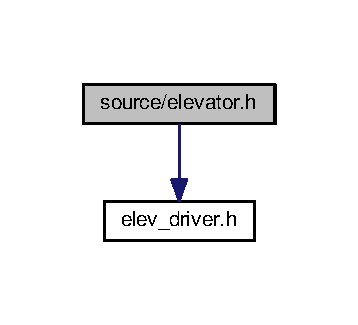
\includegraphics[width=172pt]{elevator_8h__incl}
\end{center}
\end{figure}
This graph shows which files directly or indirectly include this file\+:\nopagebreak
\begin{figure}[H]
\begin{center}
\leavevmode
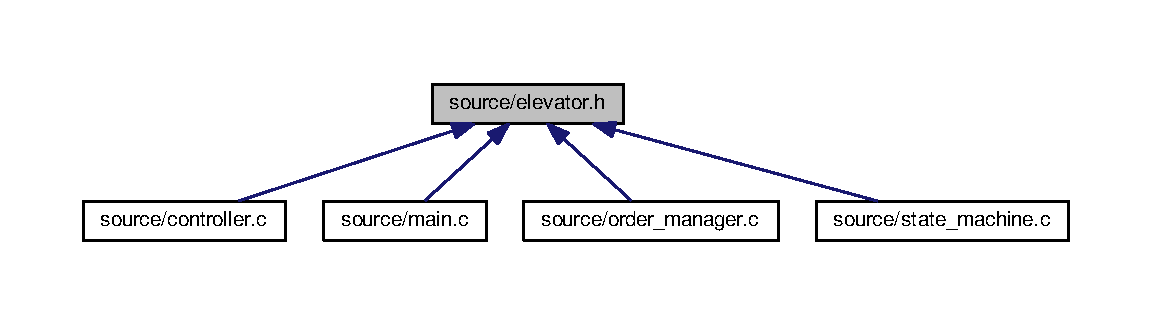
\includegraphics[width=350pt]{elevator_8h__dep__incl}
\end{center}
\end{figure}
\subsection*{Functions}
\begin{DoxyCompactItemize}
\item 
void \hyperlink{elevator_8h_a19c7b7e959f0f2621a6566df8cb7b3ba}{set\+\_\+current\+\_\+motor\+\_\+dir} (\hyperlink{elev__driver_8h_a2256dfd58fecce253106f83fd2ed607f}{elev\+\_\+motor\+\_\+direction\+\_\+t} curr\+\_\+motor\+\_\+dir)
\begin{DoxyCompactList}\small\item\em Sets {\ttfamily curr\+\_\+motor\+\_\+dir}. \end{DoxyCompactList}\item 
void \hyperlink{elevator_8h_a35063f28c57cd4c2cfe3b2d12a3a7cc3}{set\+\_\+last\+\_\+motor\+\_\+dir} (\hyperlink{elev__driver_8h_a2256dfd58fecce253106f83fd2ed607f}{elev\+\_\+motor\+\_\+direction\+\_\+t} last\+\_\+motor\+\_\+dir)
\begin{DoxyCompactList}\small\item\em Sets {\ttfamily last\+\_\+motor\+\_\+dir}. \end{DoxyCompactList}\item 
void \hyperlink{elevator_8h_a835af862b8f5f8c813437f97f5c107e0}{set\+\_\+current\+\_\+floor} (int curr\+\_\+floor)
\begin{DoxyCompactList}\small\item\em Sets {\ttfamily curr\+\_\+floor}. \end{DoxyCompactList}\item 
void \hyperlink{elevator_8h_a19b6f7e1acdb71f74ea2233560008ae1}{set\+\_\+last\+\_\+floor} (int last\+\_\+floor)
\begin{DoxyCompactList}\small\item\em Sets {\ttfamily last\+\_\+floor}. \end{DoxyCompactList}\item 
\hyperlink{elev__driver_8h_a2256dfd58fecce253106f83fd2ed607f}{elev\+\_\+motor\+\_\+direction\+\_\+t} \hyperlink{elevator_8h_a49b69d3b57f7320772b00a17bfa189be}{get\+\_\+current\+\_\+motor\+\_\+dir} ()
\begin{DoxyCompactList}\small\item\em Gets the elevator\textquotesingle{}s current motor direction. \end{DoxyCompactList}\item 
\hyperlink{elev__driver_8h_a2256dfd58fecce253106f83fd2ed607f}{elev\+\_\+motor\+\_\+direction\+\_\+t} \hyperlink{elevator_8h_a38d0f671c4e590729f716c236f05484e}{get\+\_\+last\+\_\+motor\+\_\+dir} ()
\begin{DoxyCompactList}\small\item\em Gets the elevator\textquotesingle{}s last motor direction. \end{DoxyCompactList}\item 
int \hyperlink{elevator_8h_a6f0d72c6372b6150b260a70e0c4ecbb5}{get\+\_\+last\+\_\+floor} ()
\begin{DoxyCompactList}\small\item\em Gets the last floor the elevator has been at. \end{DoxyCompactList}\item 
int \hyperlink{elevator_8h_a72be1591c37ccc47bcddab6e87a729b8}{get\+\_\+current\+\_\+floor} ()
\begin{DoxyCompactList}\small\item\em Gets which floor the elevator is at. \end{DoxyCompactList}\end{DoxyCompactItemize}


\subsection{Detailed Description}
Functions for getting and setting the elevators floor and motor direction. 



\subsection{Function Documentation}
\index{elevator.\+h@{elevator.\+h}!get\+\_\+current\+\_\+floor@{get\+\_\+current\+\_\+floor}}
\index{get\+\_\+current\+\_\+floor@{get\+\_\+current\+\_\+floor}!elevator.\+h@{elevator.\+h}}
\subsubsection[{\texorpdfstring{get\+\_\+current\+\_\+floor()}{get_current_floor()}}]{\setlength{\rightskip}{0pt plus 5cm}int get\+\_\+current\+\_\+floor (
\begin{DoxyParamCaption}
{}
\end{DoxyParamCaption}
)}\hypertarget{elevator_8h_a72be1591c37ccc47bcddab6e87a729b8}{}\label{elevator_8h_a72be1591c37ccc47bcddab6e87a729b8}


Gets which floor the elevator is at. 

\begin{DoxyReturn}{Returns}
current floor if elevator at floor. -\/1 if between two floors. 
\end{DoxyReturn}


Definition at line 47 of file elevator.\+c.

\index{elevator.\+h@{elevator.\+h}!get\+\_\+current\+\_\+motor\+\_\+dir@{get\+\_\+current\+\_\+motor\+\_\+dir}}
\index{get\+\_\+current\+\_\+motor\+\_\+dir@{get\+\_\+current\+\_\+motor\+\_\+dir}!elevator.\+h@{elevator.\+h}}
\subsubsection[{\texorpdfstring{get\+\_\+current\+\_\+motor\+\_\+dir()}{get_current_motor_dir()}}]{\setlength{\rightskip}{0pt plus 5cm}{\bf elev\+\_\+motor\+\_\+direction\+\_\+t} get\+\_\+current\+\_\+motor\+\_\+dir (
\begin{DoxyParamCaption}
{}
\end{DoxyParamCaption}
)}\hypertarget{elevator_8h_a49b69d3b57f7320772b00a17bfa189be}{}\label{elevator_8h_a49b69d3b57f7320772b00a17bfa189be}


Gets the elevator\textquotesingle{}s current motor direction. 

\begin{DoxyReturn}{Returns}
The elevator\textquotesingle{}s current motor direction. 
\end{DoxyReturn}


Definition at line 39 of file elevator.\+c.

\index{elevator.\+h@{elevator.\+h}!get\+\_\+last\+\_\+floor@{get\+\_\+last\+\_\+floor}}
\index{get\+\_\+last\+\_\+floor@{get\+\_\+last\+\_\+floor}!elevator.\+h@{elevator.\+h}}
\subsubsection[{\texorpdfstring{get\+\_\+last\+\_\+floor()}{get_last_floor()}}]{\setlength{\rightskip}{0pt plus 5cm}int get\+\_\+last\+\_\+floor (
\begin{DoxyParamCaption}
{}
\end{DoxyParamCaption}
)}\hypertarget{elevator_8h_a6f0d72c6372b6150b260a70e0c4ecbb5}{}\label{elevator_8h_a6f0d72c6372b6150b260a70e0c4ecbb5}


Gets the last floor the elevator has been at. 

\begin{DoxyReturn}{Returns}
last floor 
\end{DoxyReturn}


Definition at line 51 of file elevator.\+c.

\index{elevator.\+h@{elevator.\+h}!get\+\_\+last\+\_\+motor\+\_\+dir@{get\+\_\+last\+\_\+motor\+\_\+dir}}
\index{get\+\_\+last\+\_\+motor\+\_\+dir@{get\+\_\+last\+\_\+motor\+\_\+dir}!elevator.\+h@{elevator.\+h}}
\subsubsection[{\texorpdfstring{get\+\_\+last\+\_\+motor\+\_\+dir()}{get_last_motor_dir()}}]{\setlength{\rightskip}{0pt plus 5cm}{\bf elev\+\_\+motor\+\_\+direction\+\_\+t} get\+\_\+last\+\_\+motor\+\_\+dir (
\begin{DoxyParamCaption}
{}
\end{DoxyParamCaption}
)}\hypertarget{elevator_8h_a38d0f671c4e590729f716c236f05484e}{}\label{elevator_8h_a38d0f671c4e590729f716c236f05484e}


Gets the elevator\textquotesingle{}s last motor direction. 

\begin{DoxyReturn}{Returns}
The elevator\textquotesingle{}s last motor direction. 
\end{DoxyReturn}


Definition at line 43 of file elevator.\+c.

\index{elevator.\+h@{elevator.\+h}!set\+\_\+current\+\_\+floor@{set\+\_\+current\+\_\+floor}}
\index{set\+\_\+current\+\_\+floor@{set\+\_\+current\+\_\+floor}!elevator.\+h@{elevator.\+h}}
\subsubsection[{\texorpdfstring{set\+\_\+current\+\_\+floor(int curr\+\_\+floor)}{set_current_floor(int curr_floor)}}]{\setlength{\rightskip}{0pt plus 5cm}void set\+\_\+current\+\_\+floor (
\begin{DoxyParamCaption}
\item[{int}]{curr\+\_\+floor}
\end{DoxyParamCaption}
)}\hypertarget{elevator_8h_a835af862b8f5f8c813437f97f5c107e0}{}\label{elevator_8h_a835af862b8f5f8c813437f97f5c107e0}


Sets {\ttfamily curr\+\_\+floor}. 


\begin{DoxyParams}[1]{Parameters}
\mbox{\tt in}  & {\em curr\+\_\+floor} & Elevator\textquotesingle{}s current floor. \\
\hline
\end{DoxyParams}


Definition at line 31 of file elevator.\+c.

\index{elevator.\+h@{elevator.\+h}!set\+\_\+current\+\_\+motor\+\_\+dir@{set\+\_\+current\+\_\+motor\+\_\+dir}}
\index{set\+\_\+current\+\_\+motor\+\_\+dir@{set\+\_\+current\+\_\+motor\+\_\+dir}!elevator.\+h@{elevator.\+h}}
\subsubsection[{\texorpdfstring{set\+\_\+current\+\_\+motor\+\_\+dir(elev\+\_\+motor\+\_\+direction\+\_\+t curr\+\_\+motor\+\_\+dir)}{set_current_motor_dir(elev_motor_direction_t curr_motor_dir)}}]{\setlength{\rightskip}{0pt plus 5cm}void set\+\_\+current\+\_\+motor\+\_\+dir (
\begin{DoxyParamCaption}
\item[{{\bf elev\+\_\+motor\+\_\+direction\+\_\+t}}]{curr\+\_\+motor\+\_\+dir}
\end{DoxyParamCaption}
)}\hypertarget{elevator_8h_a19c7b7e959f0f2621a6566df8cb7b3ba}{}\label{elevator_8h_a19c7b7e959f0f2621a6566df8cb7b3ba}


Sets {\ttfamily curr\+\_\+motor\+\_\+dir}. 


\begin{DoxyParams}[1]{Parameters}
\mbox{\tt in}  & {\em curr\+\_\+motor\+\_\+dir} & The elevator\textquotesingle{}s current motor direction. \\
\hline
\end{DoxyParams}


Definition at line 23 of file elevator.\+c.

\index{elevator.\+h@{elevator.\+h}!set\+\_\+last\+\_\+floor@{set\+\_\+last\+\_\+floor}}
\index{set\+\_\+last\+\_\+floor@{set\+\_\+last\+\_\+floor}!elevator.\+h@{elevator.\+h}}
\subsubsection[{\texorpdfstring{set\+\_\+last\+\_\+floor(int last\+\_\+floor)}{set_last_floor(int last_floor)}}]{\setlength{\rightskip}{0pt plus 5cm}void set\+\_\+last\+\_\+floor (
\begin{DoxyParamCaption}
\item[{int}]{last\+\_\+floor}
\end{DoxyParamCaption}
)}\hypertarget{elevator_8h_a19b6f7e1acdb71f74ea2233560008ae1}{}\label{elevator_8h_a19b6f7e1acdb71f74ea2233560008ae1}


Sets {\ttfamily last\+\_\+floor}. 


\begin{DoxyParams}[1]{Parameters}
\mbox{\tt in}  & {\em last\+\_\+floor} & Elevator\textquotesingle{}s last floor. \\
\hline
\end{DoxyParams}


Definition at line 35 of file elevator.\+c.

\index{elevator.\+h@{elevator.\+h}!set\+\_\+last\+\_\+motor\+\_\+dir@{set\+\_\+last\+\_\+motor\+\_\+dir}}
\index{set\+\_\+last\+\_\+motor\+\_\+dir@{set\+\_\+last\+\_\+motor\+\_\+dir}!elevator.\+h@{elevator.\+h}}
\subsubsection[{\texorpdfstring{set\+\_\+last\+\_\+motor\+\_\+dir(elev\+\_\+motor\+\_\+direction\+\_\+t last\+\_\+motor\+\_\+dir)}{set_last_motor_dir(elev_motor_direction_t last_motor_dir)}}]{\setlength{\rightskip}{0pt plus 5cm}void set\+\_\+last\+\_\+motor\+\_\+dir (
\begin{DoxyParamCaption}
\item[{{\bf elev\+\_\+motor\+\_\+direction\+\_\+t}}]{last\+\_\+motor\+\_\+dir}
\end{DoxyParamCaption}
)}\hypertarget{elevator_8h_a35063f28c57cd4c2cfe3b2d12a3a7cc3}{}\label{elevator_8h_a35063f28c57cd4c2cfe3b2d12a3a7cc3}


Sets {\ttfamily last\+\_\+motor\+\_\+dir}. 


\begin{DoxyParams}[1]{Parameters}
\mbox{\tt in}  & {\em last\+\_\+motor\+\_\+dir} & The elevator\textquotesingle{}s last motor direction. \\
\hline
\end{DoxyParams}


Definition at line 27 of file elevator.\+c.


\hypertarget{io_8c}{}\section{source/io.c File Reference}
\label{io_8c}\index{source/io.\+c@{source/io.\+c}}
{\ttfamily \#include \char`\"{}io.\+h\char`\"{}}\\*
{\ttfamily \#include \char`\"{}channels.\+h\char`\"{}}\\*
{\ttfamily \#include $<$comedilib.\+h$>$}\\*
Include dependency graph for io.\+c\+:
\nopagebreak
\begin{figure}[H]
\begin{center}
\leavevmode
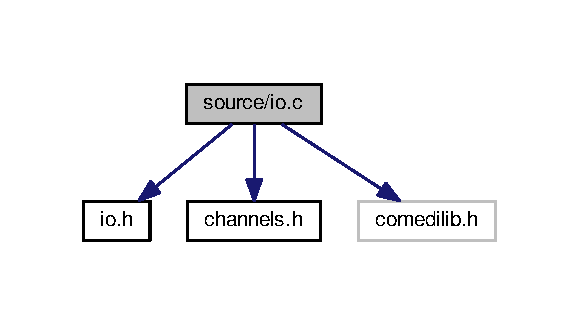
\includegraphics[width=278pt]{io_8c__incl}
\end{center}
\end{figure}
\subsection*{Functions}
\begin{DoxyCompactItemize}
\item 
int \hyperlink{io_8c_a12ce98b64f2019ac45b44826a4db7ec9}{io\+\_\+init} ()
\item 
void \hyperlink{io_8c_a4d538858b80ee856217e3ecfde8a3c60}{io\+\_\+set\+\_\+bit} (int channel)
\item 
void \hyperlink{io_8c_a97951257634a0778b858a4ced7558f81}{io\+\_\+clear\+\_\+bit} (int channel)
\item 
void \hyperlink{io_8c_a1c2c5df63111187109ef11be354621bd}{io\+\_\+write\+\_\+analog} (int channel, int value)
\item 
int \hyperlink{io_8c_ae9e08ee7d41b07b153e2ddaae4dc53cb}{io\+\_\+read\+\_\+bit} (int channel)
\item 
int \hyperlink{io_8c_ab145a5637d2c463dfb5741e1a748dd74}{io\+\_\+read\+\_\+analog} (int channel)
\end{DoxyCompactItemize}


\subsection{Function Documentation}
\index{io.\+c@{io.\+c}!io\+\_\+clear\+\_\+bit@{io\+\_\+clear\+\_\+bit}}
\index{io\+\_\+clear\+\_\+bit@{io\+\_\+clear\+\_\+bit}!io.\+c@{io.\+c}}
\subsubsection[{\texorpdfstring{io\+\_\+clear\+\_\+bit(int channel)}{io_clear_bit(int channel)}}]{\setlength{\rightskip}{0pt plus 5cm}void io\+\_\+clear\+\_\+bit (
\begin{DoxyParamCaption}
\item[{int}]{channel}
\end{DoxyParamCaption}
)}\hypertarget{io_8c_a97951257634a0778b858a4ced7558f81}{}\label{io_8c_a97951257634a0778b858a4ced7558f81}
Clears a digital channel bit. 
\begin{DoxyParams}{Parameters}
{\em channel} & Channel bit to set. \\
\hline
\end{DoxyParams}


Definition at line 47 of file io.\+c.

\index{io.\+c@{io.\+c}!io\+\_\+init@{io\+\_\+init}}
\index{io\+\_\+init@{io\+\_\+init}!io.\+c@{io.\+c}}
\subsubsection[{\texorpdfstring{io\+\_\+init()}{io_init()}}]{\setlength{\rightskip}{0pt plus 5cm}int io\+\_\+init (
\begin{DoxyParamCaption}
{}
\end{DoxyParamCaption}
)}\hypertarget{io_8c_a12ce98b64f2019ac45b44826a4db7ec9}{}\label{io_8c_a12ce98b64f2019ac45b44826a4db7ec9}
Initialize lib\+Comedi in \char`\"{}\+Sanntidssalen\char`\"{} \begin{DoxyReturn}{Returns}
Non-\/zero on success and 0 on failure 
\end{DoxyReturn}


Definition at line 20 of file io.\+c.

\index{io.\+c@{io.\+c}!io\+\_\+read\+\_\+analog@{io\+\_\+read\+\_\+analog}}
\index{io\+\_\+read\+\_\+analog@{io\+\_\+read\+\_\+analog}!io.\+c@{io.\+c}}
\subsubsection[{\texorpdfstring{io\+\_\+read\+\_\+analog(int channel)}{io_read_analog(int channel)}}]{\setlength{\rightskip}{0pt plus 5cm}int io\+\_\+read\+\_\+analog (
\begin{DoxyParamCaption}
\item[{int}]{channel}
\end{DoxyParamCaption}
)}\hypertarget{io_8c_ab145a5637d2c463dfb5741e1a748dd74}{}\label{io_8c_ab145a5637d2c463dfb5741e1a748dd74}
Reads a bit value from an analog channel. 
\begin{DoxyParams}{Parameters}
{\em channel} & Channel to read from. \\
\hline
\end{DoxyParams}
\begin{DoxyReturn}{Returns}
Value read. 
\end{DoxyReturn}


Definition at line 68 of file io.\+c.

\index{io.\+c@{io.\+c}!io\+\_\+read\+\_\+bit@{io\+\_\+read\+\_\+bit}}
\index{io\+\_\+read\+\_\+bit@{io\+\_\+read\+\_\+bit}!io.\+c@{io.\+c}}
\subsubsection[{\texorpdfstring{io\+\_\+read\+\_\+bit(int channel)}{io_read_bit(int channel)}}]{\setlength{\rightskip}{0pt plus 5cm}int io\+\_\+read\+\_\+bit (
\begin{DoxyParamCaption}
\item[{int}]{channel}
\end{DoxyParamCaption}
)}\hypertarget{io_8c_ae9e08ee7d41b07b153e2ddaae4dc53cb}{}\label{io_8c_ae9e08ee7d41b07b153e2ddaae4dc53cb}
Reads a bit value from a digital channel. 
\begin{DoxyParams}{Parameters}
{\em channel} & Channel to read from. \\
\hline
\end{DoxyParams}
\begin{DoxyReturn}{Returns}
Value read. 
\end{DoxyReturn}


Definition at line 59 of file io.\+c.

\index{io.\+c@{io.\+c}!io\+\_\+set\+\_\+bit@{io\+\_\+set\+\_\+bit}}
\index{io\+\_\+set\+\_\+bit@{io\+\_\+set\+\_\+bit}!io.\+c@{io.\+c}}
\subsubsection[{\texorpdfstring{io\+\_\+set\+\_\+bit(int channel)}{io_set_bit(int channel)}}]{\setlength{\rightskip}{0pt plus 5cm}void io\+\_\+set\+\_\+bit (
\begin{DoxyParamCaption}
\item[{int}]{channel}
\end{DoxyParamCaption}
)}\hypertarget{io_8c_a4d538858b80ee856217e3ecfde8a3c60}{}\label{io_8c_a4d538858b80ee856217e3ecfde8a3c60}
Sets a digital channel bit. 
\begin{DoxyParams}{Parameters}
{\em channel} & Channel bit to set. \\
\hline
\end{DoxyParams}


Definition at line 41 of file io.\+c.

\index{io.\+c@{io.\+c}!io\+\_\+write\+\_\+analog@{io\+\_\+write\+\_\+analog}}
\index{io\+\_\+write\+\_\+analog@{io\+\_\+write\+\_\+analog}!io.\+c@{io.\+c}}
\subsubsection[{\texorpdfstring{io\+\_\+write\+\_\+analog(int channel, int value)}{io_write_analog(int channel, int value)}}]{\setlength{\rightskip}{0pt plus 5cm}void io\+\_\+write\+\_\+analog (
\begin{DoxyParamCaption}
\item[{int}]{channel, }
\item[{int}]{value}
\end{DoxyParamCaption}
)}\hypertarget{io_8c_a1c2c5df63111187109ef11be354621bd}{}\label{io_8c_a1c2c5df63111187109ef11be354621bd}
Writes a value to an analog channel. 
\begin{DoxyParams}{Parameters}
{\em channel} & Channel to write to. \\
\hline
{\em value} & Value to write. \\
\hline
\end{DoxyParams}


Definition at line 53 of file io.\+c.


\hypertarget{io_8h}{}\section{source/io.h File Reference}
\label{io_8h}\index{source/io.\+h@{source/io.\+h}}


Implementation file for io.  


This graph shows which files directly or indirectly include this file\+:\nopagebreak
\begin{figure}[H]
\begin{center}
\leavevmode
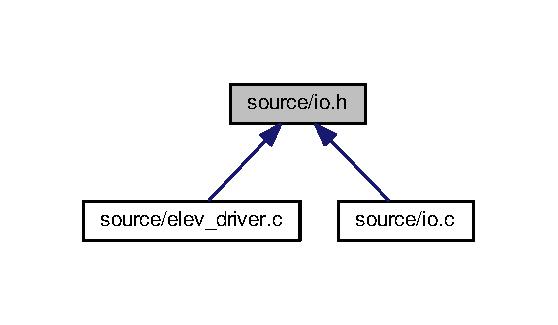
\includegraphics[width=268pt]{io_8h__dep__incl}
\end{center}
\end{figure}
\subsection*{Functions}
\begin{DoxyCompactItemize}
\item 
int \hyperlink{io_8h_a12ce98b64f2019ac45b44826a4db7ec9}{io\+\_\+init} ()
\item 
void \hyperlink{io_8h_a4d538858b80ee856217e3ecfde8a3c60}{io\+\_\+set\+\_\+bit} (int channel)
\item 
void \hyperlink{io_8h_a97951257634a0778b858a4ced7558f81}{io\+\_\+clear\+\_\+bit} (int channel)
\item 
void \hyperlink{io_8h_a1c2c5df63111187109ef11be354621bd}{io\+\_\+write\+\_\+analog} (int channel, int value)
\item 
int \hyperlink{io_8h_ae9e08ee7d41b07b153e2ddaae4dc53cb}{io\+\_\+read\+\_\+bit} (int channel)
\item 
int \hyperlink{io_8h_ab145a5637d2c463dfb5741e1a748dd74}{io\+\_\+read\+\_\+analog} (int channel)
\end{DoxyCompactItemize}


\subsection{Detailed Description}
Implementation file for io. 



\subsection{Function Documentation}
\index{io.\+h@{io.\+h}!io\+\_\+clear\+\_\+bit@{io\+\_\+clear\+\_\+bit}}
\index{io\+\_\+clear\+\_\+bit@{io\+\_\+clear\+\_\+bit}!io.\+h@{io.\+h}}
\subsubsection[{\texorpdfstring{io\+\_\+clear\+\_\+bit(int channel)}{io_clear_bit(int channel)}}]{\setlength{\rightskip}{0pt plus 5cm}void io\+\_\+clear\+\_\+bit (
\begin{DoxyParamCaption}
\item[{int}]{channel}
\end{DoxyParamCaption}
)}\hypertarget{io_8h_a97951257634a0778b858a4ced7558f81}{}\label{io_8h_a97951257634a0778b858a4ced7558f81}
Clears a digital channel bit. 
\begin{DoxyParams}{Parameters}
{\em channel} & Channel bit to set. \\
\hline
\end{DoxyParams}


Definition at line 48 of file io.\+c.

\index{io.\+h@{io.\+h}!io\+\_\+init@{io\+\_\+init}}
\index{io\+\_\+init@{io\+\_\+init}!io.\+h@{io.\+h}}
\subsubsection[{\texorpdfstring{io\+\_\+init()}{io_init()}}]{\setlength{\rightskip}{0pt plus 5cm}int io\+\_\+init (
\begin{DoxyParamCaption}
{}
\end{DoxyParamCaption}
)}\hypertarget{io_8h_a12ce98b64f2019ac45b44826a4db7ec9}{}\label{io_8h_a12ce98b64f2019ac45b44826a4db7ec9}
Initialize lib\+Comedi in \char`\"{}\+Sanntidssalen\char`\"{} \begin{DoxyReturn}{Returns}
Non-\/zero on success and 0 on failure 
\end{DoxyReturn}


Definition at line 21 of file io.\+c.

\index{io.\+h@{io.\+h}!io\+\_\+read\+\_\+analog@{io\+\_\+read\+\_\+analog}}
\index{io\+\_\+read\+\_\+analog@{io\+\_\+read\+\_\+analog}!io.\+h@{io.\+h}}
\subsubsection[{\texorpdfstring{io\+\_\+read\+\_\+analog(int channel)}{io_read_analog(int channel)}}]{\setlength{\rightskip}{0pt plus 5cm}int io\+\_\+read\+\_\+analog (
\begin{DoxyParamCaption}
\item[{int}]{channel}
\end{DoxyParamCaption}
)}\hypertarget{io_8h_ab145a5637d2c463dfb5741e1a748dd74}{}\label{io_8h_ab145a5637d2c463dfb5741e1a748dd74}
Reads a bit value from an analog channel. 
\begin{DoxyParams}{Parameters}
{\em channel} & Channel to read from. \\
\hline
\end{DoxyParams}
\begin{DoxyReturn}{Returns}
Value read. 
\end{DoxyReturn}


Definition at line 69 of file io.\+c.

\index{io.\+h@{io.\+h}!io\+\_\+read\+\_\+bit@{io\+\_\+read\+\_\+bit}}
\index{io\+\_\+read\+\_\+bit@{io\+\_\+read\+\_\+bit}!io.\+h@{io.\+h}}
\subsubsection[{\texorpdfstring{io\+\_\+read\+\_\+bit(int channel)}{io_read_bit(int channel)}}]{\setlength{\rightskip}{0pt plus 5cm}int io\+\_\+read\+\_\+bit (
\begin{DoxyParamCaption}
\item[{int}]{channel}
\end{DoxyParamCaption}
)}\hypertarget{io_8h_ae9e08ee7d41b07b153e2ddaae4dc53cb}{}\label{io_8h_ae9e08ee7d41b07b153e2ddaae4dc53cb}
Reads a bit value from a digital channel. 
\begin{DoxyParams}{Parameters}
{\em channel} & Channel to read from. \\
\hline
\end{DoxyParams}
\begin{DoxyReturn}{Returns}
Value read. 
\end{DoxyReturn}


Definition at line 60 of file io.\+c.

\index{io.\+h@{io.\+h}!io\+\_\+set\+\_\+bit@{io\+\_\+set\+\_\+bit}}
\index{io\+\_\+set\+\_\+bit@{io\+\_\+set\+\_\+bit}!io.\+h@{io.\+h}}
\subsubsection[{\texorpdfstring{io\+\_\+set\+\_\+bit(int channel)}{io_set_bit(int channel)}}]{\setlength{\rightskip}{0pt plus 5cm}void io\+\_\+set\+\_\+bit (
\begin{DoxyParamCaption}
\item[{int}]{channel}
\end{DoxyParamCaption}
)}\hypertarget{io_8h_a4d538858b80ee856217e3ecfde8a3c60}{}\label{io_8h_a4d538858b80ee856217e3ecfde8a3c60}
Sets a digital channel bit. 
\begin{DoxyParams}{Parameters}
{\em channel} & Channel bit to set. \\
\hline
\end{DoxyParams}


Definition at line 42 of file io.\+c.

\index{io.\+h@{io.\+h}!io\+\_\+write\+\_\+analog@{io\+\_\+write\+\_\+analog}}
\index{io\+\_\+write\+\_\+analog@{io\+\_\+write\+\_\+analog}!io.\+h@{io.\+h}}
\subsubsection[{\texorpdfstring{io\+\_\+write\+\_\+analog(int channel, int value)}{io_write_analog(int channel, int value)}}]{\setlength{\rightskip}{0pt plus 5cm}void io\+\_\+write\+\_\+analog (
\begin{DoxyParamCaption}
\item[{int}]{channel, }
\item[{int}]{value}
\end{DoxyParamCaption}
)}\hypertarget{io_8h_a1c2c5df63111187109ef11be354621bd}{}\label{io_8h_a1c2c5df63111187109ef11be354621bd}
Writes a value to an analog channel. 
\begin{DoxyParams}{Parameters}
{\em channel} & Channel to write to. \\
\hline
{\em value} & Value to write. \\
\hline
\end{DoxyParams}


Definition at line 54 of file io.\+c.


\hypertarget{order__manager_8c}{}\section{source/order\+\_\+manager.c File Reference}
\label{order__manager_8c}\index{source/order\+\_\+manager.\+c@{source/order\+\_\+manager.\+c}}
{\ttfamily \#include \char`\"{}order\+\_\+manager.\+h\char`\"{}}\\*
{\ttfamily \#include \char`\"{}elev\+\_\+driver.\+h\char`\"{}}\\*
{\ttfamily \#include \char`\"{}elevator.\+h\char`\"{}}\\*
{\ttfamily \#include $<$stdio.\+h$>$}\\*
Include dependency graph for order\+\_\+manager.\+c\+:
\nopagebreak
\begin{figure}[H]
\begin{center}
\leavevmode
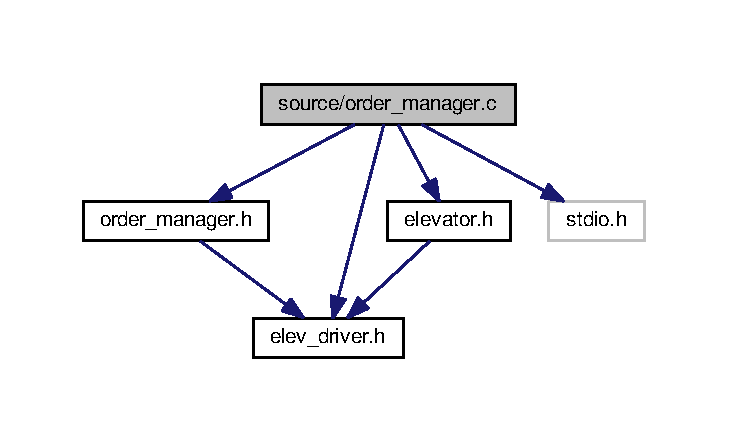
\includegraphics[width=350pt]{order__manager_8c__incl}
\end{center}
\end{figure}
\subsection*{Functions}
\begin{DoxyCompactItemize}
\item 
void \hyperlink{order__manager_8c_a8adafbbff4884372d6ffdd1ed7c60fa9}{init\+\_\+orderlist} ()\hypertarget{order__manager_8c_a8adafbbff4884372d6ffdd1ed7c60fa9}{}\label{order__manager_8c_a8adafbbff4884372d6ffdd1ed7c60fa9}

\begin{DoxyCompactList}\small\item\em Intialize a list of orders and sets all orders to be inactive. \end{DoxyCompactList}\item 
void \hyperlink{order__manager_8c_a6206e5203639ca23d84820e2ffb108a3}{clear\+\_\+all\+\_\+orders} ()\hypertarget{order__manager_8c_a6206e5203639ca23d84820e2ffb108a3}{}\label{order__manager_8c_a6206e5203639ca23d84820e2ffb108a3}

\begin{DoxyCompactList}\small\item\em Sets all orders to be inactive. \end{DoxyCompactList}\item 
void \hyperlink{order__manager_8c_ac402b78b33fb15a5593ba68dbb320fe6}{clear\+\_\+all\+\_\+orders\+\_\+at\+\_\+floor} (int floor)
\begin{DoxyCompactList}\small\item\em Sets all orders at {\ttfamily floor} to inactive and updates button lights. \end{DoxyCompactList}\item 
void \hyperlink{order__manager_8c_ad8979de5df4ed8a898d1b837b540c22d}{set\+\_\+order} (int floor, \hyperlink{elev__driver_8h_af61c4136fb437a2c49037e5a57c9abda}{elev\+\_\+button\+\_\+type\+\_\+t} button\+\_\+type)
\begin{DoxyCompactList}\small\item\em Sets an order to active and updates order lights. \end{DoxyCompactList}\item 
\hyperlink{order__manager_8h_a88b083f4969e7c61a34a7231180f9e41}{order} \hyperlink{order__manager_8c_a420ca28e5032b3230bafbbf100fba504}{get\+\_\+order} (int floor, \hyperlink{elev__driver_8h_af61c4136fb437a2c49037e5a57c9abda}{elev\+\_\+button\+\_\+type\+\_\+t} button\+\_\+type)
\begin{DoxyCompactList}\small\item\em Gets order given by {\ttfamily floor} and . \end{DoxyCompactList}\item 
int \hyperlink{order__manager_8c_aead0bede1788c3c3050dc49a7e191382}{orders\+\_\+above} (int current\+\_\+floor)
\begin{DoxyCompactList}\small\item\em Checks if it is any orders above {\ttfamily current\+\_\+floor}. \end{DoxyCompactList}\item 
int \hyperlink{order__manager_8c_a704d50341b06a68154a6e4bcdf950c31}{orders\+\_\+below} (int current\+\_\+floor)
\begin{DoxyCompactList}\small\item\em Checks if it is any orders below {\ttfamily current\+\_\+floor}. \end{DoxyCompactList}\item 
int \hyperlink{order__manager_8c_acd80fbd88c2b6735f067f5fc564e3201}{is\+\_\+active\+\_\+orders} ()
\begin{DoxyCompactList}\small\item\em Goes through the Orderlist and checks if it is any active orders. \end{DoxyCompactList}\item 
int \hyperlink{order__manager_8c_ae574e8525583cfbb6adc9e7f32548d1c}{is\+\_\+order\+\_\+at\+\_\+floor} (int floor, \hyperlink{elev__driver_8h_a2256dfd58fecce253106f83fd2ed607f}{elev\+\_\+motor\+\_\+direction\+\_\+t} motor\+\_\+dir)
\begin{DoxyCompactList}\small\item\em Checks if an order is at a given floor and if the elevator should stop. The elevator should only stop if the elevator\textquotesingle{}s motor direction and order is in the same direction. \end{DoxyCompactList}\item 
void \hyperlink{order__manager_8c_aed99ef2613ad95a6d5905fa21ca145ef}{update\+\_\+button\+\_\+lights} ()\hypertarget{order__manager_8c_aed99ef2613ad95a6d5905fa21ca145ef}{}\label{order__manager_8c_aed99ef2613ad95a6d5905fa21ca145ef}

\begin{DoxyCompactList}\small\item\em Updates button lights. Turns off lights if order at floor is completed. \end{DoxyCompactList}\end{DoxyCompactItemize}
\subsection*{Variables}
\begin{DoxyCompactItemize}
\item 
\hyperlink{order__manager_8h_a88b083f4969e7c61a34a7231180f9e41}{order} {\bfseries Orderlist} \mbox{[}N\+\_\+\+F\+L\+O\+O\+RS\mbox{]}\mbox{[}N\+\_\+\+B\+U\+T\+T\+O\+NS\mbox{]}\hypertarget{order__manager_8c_aa132bb6c8c37af1662af4632dcda435a}{}\label{order__manager_8c_aa132bb6c8c37af1662af4632dcda435a}

\end{DoxyCompactItemize}


\subsection{Function Documentation}
\index{order\+\_\+manager.\+c@{order\+\_\+manager.\+c}!clear\+\_\+all\+\_\+orders\+\_\+at\+\_\+floor@{clear\+\_\+all\+\_\+orders\+\_\+at\+\_\+floor}}
\index{clear\+\_\+all\+\_\+orders\+\_\+at\+\_\+floor@{clear\+\_\+all\+\_\+orders\+\_\+at\+\_\+floor}!order\+\_\+manager.\+c@{order\+\_\+manager.\+c}}
\subsubsection[{\texorpdfstring{clear\+\_\+all\+\_\+orders\+\_\+at\+\_\+floor(int floor)}{clear_all_orders_at_floor(int floor)}}]{\setlength{\rightskip}{0pt plus 5cm}void clear\+\_\+all\+\_\+orders\+\_\+at\+\_\+floor (
\begin{DoxyParamCaption}
\item[{int}]{floor}
\end{DoxyParamCaption}
)}\hypertarget{order__manager_8c_ac402b78b33fb15a5593ba68dbb320fe6}{}\label{order__manager_8c_ac402b78b33fb15a5593ba68dbb320fe6}


Sets all orders at {\ttfamily floor} to inactive and updates button lights. 


\begin{DoxyParams}[1]{Parameters}
\mbox{\tt in}  & {\em floor} & The floor you want to clear all orders at. \\
\hline
\end{DoxyParams}


Definition at line 27 of file order\+\_\+manager.\+c.

\index{order\+\_\+manager.\+c@{order\+\_\+manager.\+c}!get\+\_\+order@{get\+\_\+order}}
\index{get\+\_\+order@{get\+\_\+order}!order\+\_\+manager.\+c@{order\+\_\+manager.\+c}}
\subsubsection[{\texorpdfstring{get\+\_\+order(int floor, elev\+\_\+button\+\_\+type\+\_\+t button\+\_\+type)}{get_order(int floor, elev_button_type_t button_type)}}]{\setlength{\rightskip}{0pt plus 5cm}{\bf order} get\+\_\+order (
\begin{DoxyParamCaption}
\item[{int}]{floor, }
\item[{{\bf elev\+\_\+button\+\_\+type\+\_\+t}}]{button\+\_\+type}
\end{DoxyParamCaption}
)}\hypertarget{order__manager_8c_a420ca28e5032b3230bafbbf100fba504}{}\label{order__manager_8c_a420ca28e5032b3230bafbbf100fba504}


Gets order given by {\ttfamily floor} and . 


\begin{DoxyParams}[1]{Parameters}
\mbox{\tt in}  & {\em floor} & At which floor we want the order from. \\
\hline
\mbox{\tt in}  & {\em button\+\_\+type} & If we want the order for UP, D\+O\+WN or C\+O\+M\+M\+A\+ND.\\
\hline
\end{DoxyParams}
\begin{DoxyReturn}{Returns}
The order at the place in Orderlist given by the parameters. 
\end{DoxyReturn}


Definition at line 46 of file order\+\_\+manager.\+c.

\index{order\+\_\+manager.\+c@{order\+\_\+manager.\+c}!is\+\_\+active\+\_\+orders@{is\+\_\+active\+\_\+orders}}
\index{is\+\_\+active\+\_\+orders@{is\+\_\+active\+\_\+orders}!order\+\_\+manager.\+c@{order\+\_\+manager.\+c}}
\subsubsection[{\texorpdfstring{is\+\_\+active\+\_\+orders()}{is_active_orders()}}]{\setlength{\rightskip}{0pt plus 5cm}int is\+\_\+active\+\_\+orders (
\begin{DoxyParamCaption}
{}
\end{DoxyParamCaption}
)}\hypertarget{order__manager_8c_acd80fbd88c2b6735f067f5fc564e3201}{}\label{order__manager_8c_acd80fbd88c2b6735f067f5fc564e3201}


Goes through the Orderlist and checks if it is any active orders. 

\begin{DoxyReturn}{Returns}
1 if any active orders, 0 if not. 
\end{DoxyReturn}


Definition at line 72 of file order\+\_\+manager.\+c.

\index{order\+\_\+manager.\+c@{order\+\_\+manager.\+c}!is\+\_\+order\+\_\+at\+\_\+floor@{is\+\_\+order\+\_\+at\+\_\+floor}}
\index{is\+\_\+order\+\_\+at\+\_\+floor@{is\+\_\+order\+\_\+at\+\_\+floor}!order\+\_\+manager.\+c@{order\+\_\+manager.\+c}}
\subsubsection[{\texorpdfstring{is\+\_\+order\+\_\+at\+\_\+floor(int floor, elev\+\_\+motor\+\_\+direction\+\_\+t motor\+\_\+dir)}{is_order_at_floor(int floor, elev_motor_direction_t motor_dir)}}]{\setlength{\rightskip}{0pt plus 5cm}int is\+\_\+order\+\_\+at\+\_\+floor (
\begin{DoxyParamCaption}
\item[{int}]{floor, }
\item[{{\bf elev\+\_\+motor\+\_\+direction\+\_\+t}}]{motor\+\_\+dir}
\end{DoxyParamCaption}
)}\hypertarget{order__manager_8c_ae574e8525583cfbb6adc9e7f32548d1c}{}\label{order__manager_8c_ae574e8525583cfbb6adc9e7f32548d1c}


Checks if an order is at a given floor and if the elevator should stop. The elevator should only stop if the elevator\textquotesingle{}s motor direction and order is in the same direction. 


\begin{DoxyParams}[1]{Parameters}
\mbox{\tt in}  & {\em floor} & The floor we want to check if it is any orders at. \\
\hline
\mbox{\tt in}  & {\em motor\+\_\+dir} & Motor direction of the elevator\\
\hline
\end{DoxyParams}
\begin{DoxyReturn}{Returns}
1 if it is order at floor and the elevator should stop, 0 if not. 
\end{DoxyReturn}


Definition at line 84 of file order\+\_\+manager.\+c.

\index{order\+\_\+manager.\+c@{order\+\_\+manager.\+c}!orders\+\_\+above@{orders\+\_\+above}}
\index{orders\+\_\+above@{orders\+\_\+above}!order\+\_\+manager.\+c@{order\+\_\+manager.\+c}}
\subsubsection[{\texorpdfstring{orders\+\_\+above(int current\+\_\+floor)}{orders_above(int current_floor)}}]{\setlength{\rightskip}{0pt plus 5cm}int orders\+\_\+above (
\begin{DoxyParamCaption}
\item[{int}]{current\+\_\+floor}
\end{DoxyParamCaption}
)}\hypertarget{order__manager_8c_aead0bede1788c3c3050dc49a7e191382}{}\label{order__manager_8c_aead0bede1788c3c3050dc49a7e191382}


Checks if it is any orders above {\ttfamily current\+\_\+floor}. 


\begin{DoxyParams}[1]{Parameters}
\mbox{\tt in}  & {\em current\+\_\+floor} & The floor we want to check if it is any orders above.\\
\hline
\end{DoxyParams}
\begin{DoxyReturn}{Returns}
1 if any orders above, 0 if not. 
\end{DoxyReturn}


Definition at line 50 of file order\+\_\+manager.\+c.

\index{order\+\_\+manager.\+c@{order\+\_\+manager.\+c}!orders\+\_\+below@{orders\+\_\+below}}
\index{orders\+\_\+below@{orders\+\_\+below}!order\+\_\+manager.\+c@{order\+\_\+manager.\+c}}
\subsubsection[{\texorpdfstring{orders\+\_\+below(int current\+\_\+floor)}{orders_below(int current_floor)}}]{\setlength{\rightskip}{0pt plus 5cm}int orders\+\_\+below (
\begin{DoxyParamCaption}
\item[{int}]{current\+\_\+floor}
\end{DoxyParamCaption}
)}\hypertarget{order__manager_8c_a704d50341b06a68154a6e4bcdf950c31}{}\label{order__manager_8c_a704d50341b06a68154a6e4bcdf950c31}


Checks if it is any orders below {\ttfamily current\+\_\+floor}. 


\begin{DoxyParams}[1]{Parameters}
\mbox{\tt in}  & {\em current\+\_\+floor} & The floor we want to check if it is any orders below.\\
\hline
\end{DoxyParams}
\begin{DoxyReturn}{Returns}
1 if any orders below, 0 if not. 
\end{DoxyReturn}


Definition at line 62 of file order\+\_\+manager.\+c.

\index{order\+\_\+manager.\+c@{order\+\_\+manager.\+c}!set\+\_\+order@{set\+\_\+order}}
\index{set\+\_\+order@{set\+\_\+order}!order\+\_\+manager.\+c@{order\+\_\+manager.\+c}}
\subsubsection[{\texorpdfstring{set\+\_\+order(int floor, elev\+\_\+button\+\_\+type\+\_\+t button\+\_\+type)}{set_order(int floor, elev_button_type_t button_type)}}]{\setlength{\rightskip}{0pt plus 5cm}void set\+\_\+order (
\begin{DoxyParamCaption}
\item[{int}]{floor, }
\item[{{\bf elev\+\_\+button\+\_\+type\+\_\+t}}]{button\+\_\+type}
\end{DoxyParamCaption}
)}\hypertarget{order__manager_8c_ad8979de5df4ed8a898d1b837b540c22d}{}\label{order__manager_8c_ad8979de5df4ed8a898d1b837b540c22d}


Sets an order to active and updates order lights. 


\begin{DoxyParams}[1]{Parameters}
\mbox{\tt in}  & {\em floor} & At which floor the order is at \\
\hline
\mbox{\tt in}  & {\em button\+\_\+type} & If the order is UP, D\+O\+WN or C\+O\+M\+M\+A\+ND. \\
\hline
\end{DoxyParams}


Definition at line 33 of file order\+\_\+manager.\+c.


\hypertarget{order__manager_8h}{}\section{source/order\+\_\+manager.h File Reference}
\label{order__manager_8h}\index{source/order\+\_\+manager.\+h@{source/order\+\_\+manager.\+h}}


Functions for how the elevator should handle orders.  


{\ttfamily \#include \char`\"{}elev\+\_\+driver.\+h\char`\"{}}\\*
Include dependency graph for order\+\_\+manager.\+h\+:
\nopagebreak
\begin{figure}[H]
\begin{center}
\leavevmode
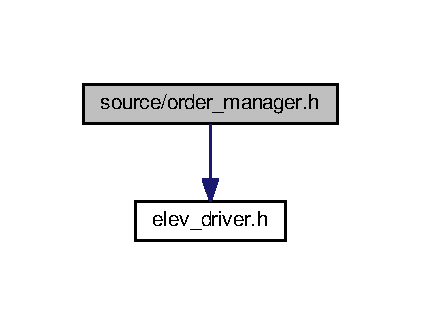
\includegraphics[width=202pt]{order__manager_8h__incl}
\end{center}
\end{figure}
This graph shows which files directly or indirectly include this file\+:
\nopagebreak
\begin{figure}[H]
\begin{center}
\leavevmode
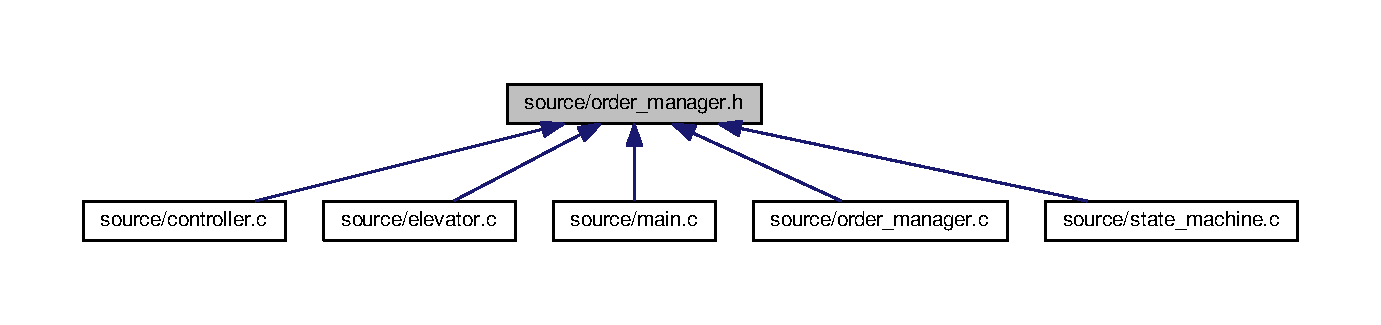
\includegraphics[width=350pt]{order__manager_8h__dep__incl}
\end{center}
\end{figure}
\subsection*{Data Structures}
\begin{DoxyCompactItemize}
\item 
struct \hyperlink{structOrder}{Order}
\end{DoxyCompactItemize}
\subsection*{Typedefs}
\begin{DoxyCompactItemize}
\item 
typedef struct \hyperlink{structOrder}{Order} \hyperlink{order__manager_8h_a88b083f4969e7c61a34a7231180f9e41}{order}
\end{DoxyCompactItemize}
\subsection*{Functions}
\begin{DoxyCompactItemize}
\item 
void \hyperlink{order__manager_8h_a8adafbbff4884372d6ffdd1ed7c60fa9}{init\+\_\+orderlist} ()\hypertarget{order__manager_8h_a8adafbbff4884372d6ffdd1ed7c60fa9}{}\label{order__manager_8h_a8adafbbff4884372d6ffdd1ed7c60fa9}

\begin{DoxyCompactList}\small\item\em Intialize a list of orders and sets all orders to be inactive. \end{DoxyCompactList}\item 
void \hyperlink{order__manager_8h_a6206e5203639ca23d84820e2ffb108a3}{clear\+\_\+all\+\_\+orders} ()\hypertarget{order__manager_8h_a6206e5203639ca23d84820e2ffb108a3}{}\label{order__manager_8h_a6206e5203639ca23d84820e2ffb108a3}

\begin{DoxyCompactList}\small\item\em Sets all orders to be inactive. \end{DoxyCompactList}\item 
void \hyperlink{order__manager_8h_ac402b78b33fb15a5593ba68dbb320fe6}{clear\+\_\+all\+\_\+orders\+\_\+at\+\_\+floor} (int floor)
\begin{DoxyCompactList}\small\item\em Sets all orders at {\ttfamily floor} to inactive and updates button lights. \end{DoxyCompactList}\item 
void \hyperlink{order__manager_8h_ad8979de5df4ed8a898d1b837b540c22d}{set\+\_\+order} (int floor, \hyperlink{elev__driver_8h_af61c4136fb437a2c49037e5a57c9abda}{elev\+\_\+button\+\_\+type\+\_\+t} button\+\_\+type)
\begin{DoxyCompactList}\small\item\em Sets an order to active and updates order lights. \end{DoxyCompactList}\item 
\hyperlink{order__manager_8h_a88b083f4969e7c61a34a7231180f9e41}{order} \hyperlink{order__manager_8h_a420ca28e5032b3230bafbbf100fba504}{get\+\_\+order} (int floor, \hyperlink{elev__driver_8h_af61c4136fb437a2c49037e5a57c9abda}{elev\+\_\+button\+\_\+type\+\_\+t} button\+\_\+type)
\begin{DoxyCompactList}\small\item\em Gets order given by {\ttfamily floor} and . \end{DoxyCompactList}\item 
int \hyperlink{order__manager_8h_aead0bede1788c3c3050dc49a7e191382}{orders\+\_\+above} (int current\+\_\+floor)
\begin{DoxyCompactList}\small\item\em Checks if it is any orders above {\ttfamily current\+\_\+floor}. \end{DoxyCompactList}\item 
int \hyperlink{order__manager_8h_a704d50341b06a68154a6e4bcdf950c31}{orders\+\_\+below} (int current\+\_\+floor)
\begin{DoxyCompactList}\small\item\em Checks if it is any orders below {\ttfamily current\+\_\+floor}. \end{DoxyCompactList}\item 
int \hyperlink{order__manager_8h_acd80fbd88c2b6735f067f5fc564e3201}{is\+\_\+active\+\_\+orders} ()
\begin{DoxyCompactList}\small\item\em Goes through the Orderlist and checks if it is any active orders. \end{DoxyCompactList}\item 
int \hyperlink{order__manager_8h_ae574e8525583cfbb6adc9e7f32548d1c}{is\+\_\+order\+\_\+at\+\_\+floor} (int floor, \hyperlink{elev__driver_8h_a2256dfd58fecce253106f83fd2ed607f}{elev\+\_\+motor\+\_\+direction\+\_\+t} motor\+\_\+dir)
\begin{DoxyCompactList}\small\item\em Checks if an order is at a given floor and if the elevator should stop. The elevator should only stop if the elevator\textquotesingle{}s motor direction and order is in the same direction. \end{DoxyCompactList}\item 
void \hyperlink{order__manager_8h_aed99ef2613ad95a6d5905fa21ca145ef}{update\+\_\+button\+\_\+lights} ()\hypertarget{order__manager_8h_aed99ef2613ad95a6d5905fa21ca145ef}{}\label{order__manager_8h_aed99ef2613ad95a6d5905fa21ca145ef}

\begin{DoxyCompactList}\small\item\em Updates button lights. Turns off lights if order at floor is completed. \end{DoxyCompactList}\end{DoxyCompactItemize}


\subsection{Detailed Description}
Functions for how the elevator should handle orders. 



\subsection{Typedef Documentation}
\index{order\+\_\+manager.\+h@{order\+\_\+manager.\+h}!order@{order}}
\index{order@{order}!order\+\_\+manager.\+h@{order\+\_\+manager.\+h}}
\subsubsection[{\texorpdfstring{order}{order}}]{\setlength{\rightskip}{0pt plus 5cm}typedef struct {\bf Order} {\bf order}}\hypertarget{order__manager_8h_a88b083f4969e7c61a34a7231180f9e41}{}\label{order__manager_8h_a88b083f4969e7c61a34a7231180f9e41}
At which floor and what type an order is. Active says if the order has been taken or not. 

\subsection{Function Documentation}
\index{order\+\_\+manager.\+h@{order\+\_\+manager.\+h}!clear\+\_\+all\+\_\+orders\+\_\+at\+\_\+floor@{clear\+\_\+all\+\_\+orders\+\_\+at\+\_\+floor}}
\index{clear\+\_\+all\+\_\+orders\+\_\+at\+\_\+floor@{clear\+\_\+all\+\_\+orders\+\_\+at\+\_\+floor}!order\+\_\+manager.\+h@{order\+\_\+manager.\+h}}
\subsubsection[{\texorpdfstring{clear\+\_\+all\+\_\+orders\+\_\+at\+\_\+floor(int floor)}{clear_all_orders_at_floor(int floor)}}]{\setlength{\rightskip}{0pt plus 5cm}void clear\+\_\+all\+\_\+orders\+\_\+at\+\_\+floor (
\begin{DoxyParamCaption}
\item[{int}]{floor}
\end{DoxyParamCaption}
)}\hypertarget{order__manager_8h_ac402b78b33fb15a5593ba68dbb320fe6}{}\label{order__manager_8h_ac402b78b33fb15a5593ba68dbb320fe6}


Sets all orders at {\ttfamily floor} to inactive and updates button lights. 


\begin{DoxyParams}[1]{Parameters}
\mbox{\tt in}  & {\em floor} & The floor you want to clear all orders at. \\
\hline
\end{DoxyParams}


Definition at line 27 of file order\+\_\+manager.\+c.

\index{order\+\_\+manager.\+h@{order\+\_\+manager.\+h}!get\+\_\+order@{get\+\_\+order}}
\index{get\+\_\+order@{get\+\_\+order}!order\+\_\+manager.\+h@{order\+\_\+manager.\+h}}
\subsubsection[{\texorpdfstring{get\+\_\+order(int floor, elev\+\_\+button\+\_\+type\+\_\+t button\+\_\+type)}{get_order(int floor, elev_button_type_t button_type)}}]{\setlength{\rightskip}{0pt plus 5cm}{\bf order} get\+\_\+order (
\begin{DoxyParamCaption}
\item[{int}]{floor, }
\item[{{\bf elev\+\_\+button\+\_\+type\+\_\+t}}]{button\+\_\+type}
\end{DoxyParamCaption}
)}\hypertarget{order__manager_8h_a420ca28e5032b3230bafbbf100fba504}{}\label{order__manager_8h_a420ca28e5032b3230bafbbf100fba504}


Gets order given by {\ttfamily floor} and . 


\begin{DoxyParams}[1]{Parameters}
\mbox{\tt in}  & {\em floor} & At which floor we want the order from. \\
\hline
\mbox{\tt in}  & {\em button\+\_\+type} & If we want the order for UP, D\+O\+WN or C\+O\+M\+M\+A\+ND.\\
\hline
\end{DoxyParams}
\begin{DoxyReturn}{Returns}
The order at the place in Orderlist given by the parameters. 
\end{DoxyReturn}


Definition at line 46 of file order\+\_\+manager.\+c.

\index{order\+\_\+manager.\+h@{order\+\_\+manager.\+h}!is\+\_\+active\+\_\+orders@{is\+\_\+active\+\_\+orders}}
\index{is\+\_\+active\+\_\+orders@{is\+\_\+active\+\_\+orders}!order\+\_\+manager.\+h@{order\+\_\+manager.\+h}}
\subsubsection[{\texorpdfstring{is\+\_\+active\+\_\+orders()}{is_active_orders()}}]{\setlength{\rightskip}{0pt plus 5cm}int is\+\_\+active\+\_\+orders (
\begin{DoxyParamCaption}
{}
\end{DoxyParamCaption}
)}\hypertarget{order__manager_8h_acd80fbd88c2b6735f067f5fc564e3201}{}\label{order__manager_8h_acd80fbd88c2b6735f067f5fc564e3201}


Goes through the Orderlist and checks if it is any active orders. 

\begin{DoxyReturn}{Returns}
1 if any active orders, 0 if not. 
\end{DoxyReturn}


Definition at line 72 of file order\+\_\+manager.\+c.

\index{order\+\_\+manager.\+h@{order\+\_\+manager.\+h}!is\+\_\+order\+\_\+at\+\_\+floor@{is\+\_\+order\+\_\+at\+\_\+floor}}
\index{is\+\_\+order\+\_\+at\+\_\+floor@{is\+\_\+order\+\_\+at\+\_\+floor}!order\+\_\+manager.\+h@{order\+\_\+manager.\+h}}
\subsubsection[{\texorpdfstring{is\+\_\+order\+\_\+at\+\_\+floor(int floor, elev\+\_\+motor\+\_\+direction\+\_\+t motor\+\_\+dir)}{is_order_at_floor(int floor, elev_motor_direction_t motor_dir)}}]{\setlength{\rightskip}{0pt plus 5cm}int is\+\_\+order\+\_\+at\+\_\+floor (
\begin{DoxyParamCaption}
\item[{int}]{floor, }
\item[{{\bf elev\+\_\+motor\+\_\+direction\+\_\+t}}]{motor\+\_\+dir}
\end{DoxyParamCaption}
)}\hypertarget{order__manager_8h_ae574e8525583cfbb6adc9e7f32548d1c}{}\label{order__manager_8h_ae574e8525583cfbb6adc9e7f32548d1c}


Checks if an order is at a given floor and if the elevator should stop. The elevator should only stop if the elevator\textquotesingle{}s motor direction and order is in the same direction. 


\begin{DoxyParams}[1]{Parameters}
\mbox{\tt in}  & {\em floor} & The floor we want to check if it is any orders at. \\
\hline
\mbox{\tt in}  & {\em motor\+\_\+dir} & Motor direction of the elevator\\
\hline
\end{DoxyParams}
\begin{DoxyReturn}{Returns}
1 if it is order at floor and the elevator should stop, 0 if not. 
\end{DoxyReturn}


Definition at line 84 of file order\+\_\+manager.\+c.

\index{order\+\_\+manager.\+h@{order\+\_\+manager.\+h}!orders\+\_\+above@{orders\+\_\+above}}
\index{orders\+\_\+above@{orders\+\_\+above}!order\+\_\+manager.\+h@{order\+\_\+manager.\+h}}
\subsubsection[{\texorpdfstring{orders\+\_\+above(int current\+\_\+floor)}{orders_above(int current_floor)}}]{\setlength{\rightskip}{0pt plus 5cm}int orders\+\_\+above (
\begin{DoxyParamCaption}
\item[{int}]{current\+\_\+floor}
\end{DoxyParamCaption}
)}\hypertarget{order__manager_8h_aead0bede1788c3c3050dc49a7e191382}{}\label{order__manager_8h_aead0bede1788c3c3050dc49a7e191382}


Checks if it is any orders above {\ttfamily current\+\_\+floor}. 


\begin{DoxyParams}[1]{Parameters}
\mbox{\tt in}  & {\em current\+\_\+floor} & The floor we want to check if it is any orders above.\\
\hline
\end{DoxyParams}
\begin{DoxyReturn}{Returns}
1 if any orders above, 0 if not. 
\end{DoxyReturn}


Definition at line 50 of file order\+\_\+manager.\+c.

\index{order\+\_\+manager.\+h@{order\+\_\+manager.\+h}!orders\+\_\+below@{orders\+\_\+below}}
\index{orders\+\_\+below@{orders\+\_\+below}!order\+\_\+manager.\+h@{order\+\_\+manager.\+h}}
\subsubsection[{\texorpdfstring{orders\+\_\+below(int current\+\_\+floor)}{orders_below(int current_floor)}}]{\setlength{\rightskip}{0pt plus 5cm}int orders\+\_\+below (
\begin{DoxyParamCaption}
\item[{int}]{current\+\_\+floor}
\end{DoxyParamCaption}
)}\hypertarget{order__manager_8h_a704d50341b06a68154a6e4bcdf950c31}{}\label{order__manager_8h_a704d50341b06a68154a6e4bcdf950c31}


Checks if it is any orders below {\ttfamily current\+\_\+floor}. 


\begin{DoxyParams}[1]{Parameters}
\mbox{\tt in}  & {\em current\+\_\+floor} & The floor we want to check if it is any orders below.\\
\hline
\end{DoxyParams}
\begin{DoxyReturn}{Returns}
1 if any orders below, 0 if not. 
\end{DoxyReturn}


Definition at line 62 of file order\+\_\+manager.\+c.

\index{order\+\_\+manager.\+h@{order\+\_\+manager.\+h}!set\+\_\+order@{set\+\_\+order}}
\index{set\+\_\+order@{set\+\_\+order}!order\+\_\+manager.\+h@{order\+\_\+manager.\+h}}
\subsubsection[{\texorpdfstring{set\+\_\+order(int floor, elev\+\_\+button\+\_\+type\+\_\+t button\+\_\+type)}{set_order(int floor, elev_button_type_t button_type)}}]{\setlength{\rightskip}{0pt plus 5cm}void set\+\_\+order (
\begin{DoxyParamCaption}
\item[{int}]{floor, }
\item[{{\bf elev\+\_\+button\+\_\+type\+\_\+t}}]{button\+\_\+type}
\end{DoxyParamCaption}
)}\hypertarget{order__manager_8h_ad8979de5df4ed8a898d1b837b540c22d}{}\label{order__manager_8h_ad8979de5df4ed8a898d1b837b540c22d}


Sets an order to active and updates order lights. 


\begin{DoxyParams}[1]{Parameters}
\mbox{\tt in}  & {\em floor} & At which floor the order is at \\
\hline
\mbox{\tt in}  & {\em button\+\_\+type} & If the order is UP, D\+O\+WN or C\+O\+M\+M\+A\+ND. \\
\hline
\end{DoxyParams}


Definition at line 33 of file order\+\_\+manager.\+c.


\hypertarget{state__machine_8h}{}\section{source/state\+\_\+machine.h File Reference}
\label{state__machine_8h}\index{source/state\+\_\+machine.\+h@{source/state\+\_\+machine.\+h}}


Functions for the state of the elevator.  


{\ttfamily \#include \char`\"{}elev\+\_\+driver.\+h\char`\"{}}\\*
Include dependency graph for state\+\_\+machine.\+h\+:\nopagebreak
\begin{figure}[H]
\begin{center}
\leavevmode
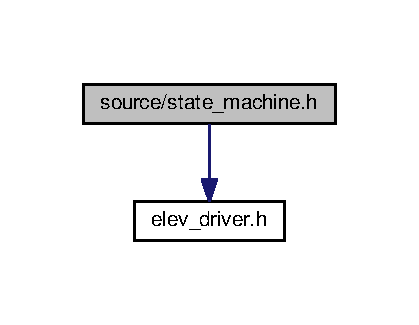
\includegraphics[width=201pt]{state__machine_8h__incl}
\end{center}
\end{figure}
This graph shows which files directly or indirectly include this file\+:\nopagebreak
\begin{figure}[H]
\begin{center}
\leavevmode
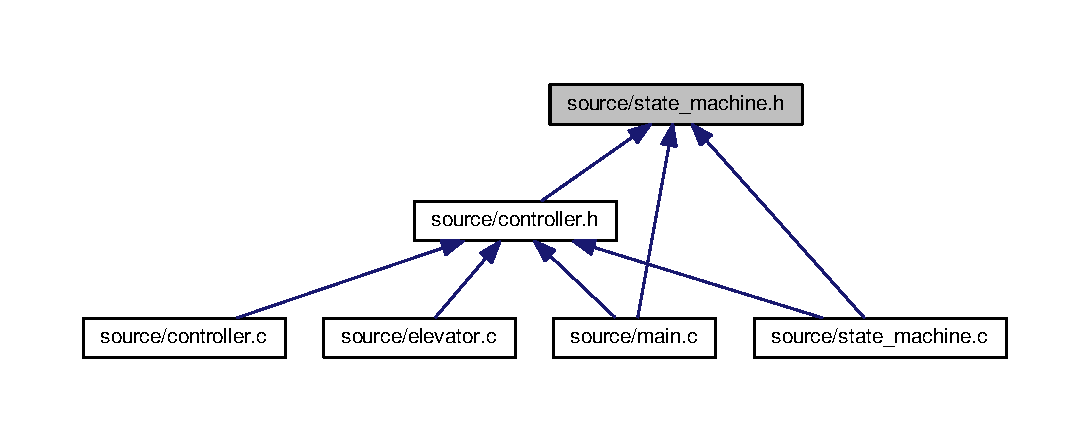
\includegraphics[width=350pt]{state__machine_8h__dep__incl}
\end{center}
\end{figure}
\subsection*{Typedefs}
\begin{DoxyCompactItemize}
\item 
typedef enum State {\bfseries state}\hypertarget{state__machine_8h_ae3081d55e54214abe932e6c511d6cac2}{}\label{state__machine_8h_ae3081d55e54214abe932e6c511d6cac2}

\end{DoxyCompactItemize}
\subsection*{Enumerations}
\begin{DoxyCompactItemize}
\item 
enum {\bfseries State} \{ \\*
{\bfseries M\+O\+V\+I\+NG}, 
{\bfseries I\+D\+LE}, 
{\bfseries D\+O\+O\+R\+\_\+\+O\+P\+EN}, 
{\bfseries S\+T\+O\+P\+\_\+\+F\+L\+O\+OR}, 
\\*
{\bfseries S\+T\+O\+P\+\_\+\+S\+H\+A\+FT}
 \}\hypertarget{state__machine_8h_a5d74787dedbc4e11c1ab15bf487e61f8}{}\label{state__machine_8h_a5d74787dedbc4e11c1ab15bf487e61f8}

\end{DoxyCompactItemize}
\subsection*{Functions}
\begin{DoxyCompactItemize}
\item 
void \hyperlink{state__machine_8h_afcf4a6ddff16950f5c2792c5663ec1d7}{state\+\_\+init} ()\hypertarget{state__machine_8h_afcf4a6ddff16950f5c2792c5663ec1d7}{}\label{state__machine_8h_afcf4a6ddff16950f5c2792c5663ec1d7}

\begin{DoxyCompactList}\small\item\em Intialize the elevator. \end{DoxyCompactList}\item 
void \hyperlink{state__machine_8h_a2f042a2a46386e05be3f891b941edddd}{state\+\_\+idle} ()\hypertarget{state__machine_8h_a2f042a2a46386e05be3f891b941edddd}{}\label{state__machine_8h_a2f042a2a46386e05be3f891b941edddd}

\begin{DoxyCompactList}\small\item\em Sets elevator to idle. \end{DoxyCompactList}\item 
void \hyperlink{state__machine_8h_ad122f82004fadb7162d1cd98e5ffc56c}{state\+\_\+moving} (\hyperlink{elev__driver_8h_a2256dfd58fecce253106f83fd2ed607f}{elev\+\_\+motor\+\_\+direction\+\_\+t} motor\+\_\+dir)
\begin{DoxyCompactList}\small\item\em Sets elevator to move in the direction {\ttfamily motor\+\_\+dir}. \end{DoxyCompactList}\item 
void \hyperlink{state__machine_8h_aef17ceeb420a4561c8714017cd3736d7}{state\+\_\+door\+\_\+open} ()\hypertarget{state__machine_8h_aef17ceeb420a4561c8714017cd3736d7}{}\label{state__machine_8h_aef17ceeb420a4561c8714017cd3736d7}

\begin{DoxyCompactList}\small\item\em Sets state to door open. Open door for 3 seconds and delete all orders at floor. \end{DoxyCompactList}\item 
void \hyperlink{state__machine_8h_ace18059c9fdd5bd26b0846e7ee378656}{state\+\_\+\+S\+T\+O\+P\+\_\+shaft} ()\hypertarget{state__machine_8h_ace18059c9fdd5bd26b0846e7ee378656}{}\label{state__machine_8h_ace18059c9fdd5bd26b0846e7ee378656}

\begin{DoxyCompactList}\small\item\em Delete all orders and stops the elevator as long as the S\+T\+OP button is pressed between floors. \end{DoxyCompactList}\item 
void \hyperlink{state__machine_8h_a5d4de83655939e40d9268ba84bf14dac}{state\+\_\+\+S\+T\+O\+P\+\_\+floor} ()\hypertarget{state__machine_8h_a5d4de83655939e40d9268ba84bf14dac}{}\label{state__machine_8h_a5d4de83655939e40d9268ba84bf14dac}

\begin{DoxyCompactList}\small\item\em Delete all orders and stops the elevator as long as the S\+T\+OP button is pressed at a floor. \end{DoxyCompactList}\end{DoxyCompactItemize}


\subsection{Detailed Description}
Functions for the state of the elevator. 



\subsection{Function Documentation}
\index{state\+\_\+machine.\+h@{state\+\_\+machine.\+h}!state\+\_\+moving@{state\+\_\+moving}}
\index{state\+\_\+moving@{state\+\_\+moving}!state\+\_\+machine.\+h@{state\+\_\+machine.\+h}}
\subsubsection[{\texorpdfstring{state\+\_\+moving(elev\+\_\+motor\+\_\+direction\+\_\+t motor\+\_\+dir)}{state_moving(elev_motor_direction_t motor_dir)}}]{\setlength{\rightskip}{0pt plus 5cm}void state\+\_\+moving (
\begin{DoxyParamCaption}
\item[{{\bf elev\+\_\+motor\+\_\+direction\+\_\+t}}]{motor\+\_\+dir}
\end{DoxyParamCaption}
)}\hypertarget{state__machine_8h_ad122f82004fadb7162d1cd98e5ffc56c}{}\label{state__machine_8h_ad122f82004fadb7162d1cd98e5ffc56c}


Sets elevator to move in the direction {\ttfamily motor\+\_\+dir}. 


\begin{DoxyParams}{Parameters}
{\em motor\+\_\+dir} & The direction the elevator should move. \\
\hline
\end{DoxyParams}


Definition at line 36 of file state\+\_\+machine.\+c.


\hypertarget{timer_8h}{}\section{source/timer.h File Reference}
\label{timer_8h}\index{source/timer.\+h@{source/timer.\+h}}


Functions for controlling the door timer.  


{\ttfamily \#include $<$time.\+h$>$}\\*
Include dependency graph for timer.\+h\+:\nopagebreak
\begin{figure}[H]
\begin{center}
\leavevmode
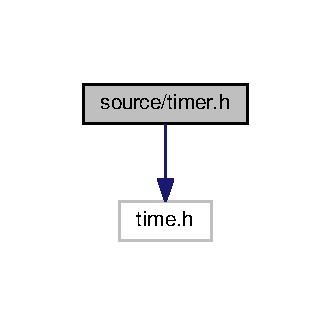
\includegraphics[width=159pt]{timer_8h__incl}
\end{center}
\end{figure}
This graph shows which files directly or indirectly include this file\+:\nopagebreak
\begin{figure}[H]
\begin{center}
\leavevmode
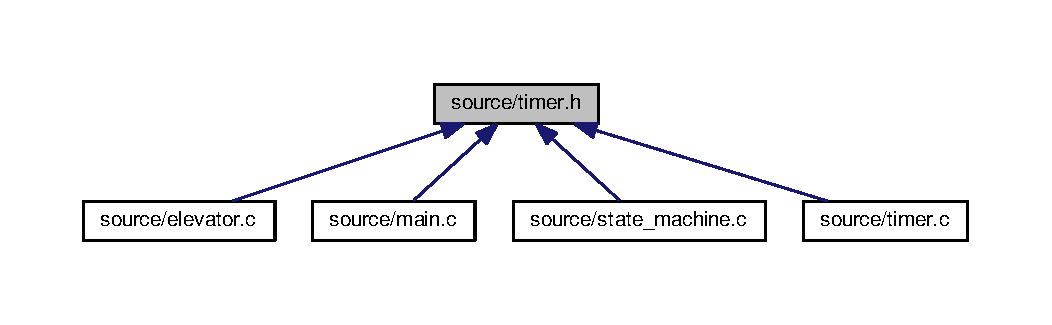
\includegraphics[width=350pt]{timer_8h__dep__incl}
\end{center}
\end{figure}
\subsection*{Functions}
\begin{DoxyCompactItemize}
\item 
void \hyperlink{timer_8h_a79cc1ad22cdc0416107de8e2ceb0d1aa}{start\+\_\+timer} (time\+\_\+t $\ast$current\+\_\+time)
\begin{DoxyCompactList}\small\item\em Starts a timer from {\ttfamily current} time. \end{DoxyCompactList}\item 
int \hyperlink{timer_8h_a9fdfb069b2978e181e0210d27bb600fa}{timer\+\_\+3\+\_\+sec} (time\+\_\+t door\+\_\+timer\+\_\+start)
\begin{DoxyCompactList}\small\item\em Counts 3 seconds from {\ttfamily door\+\_\+timer\+\_\+start}. \end{DoxyCompactList}\end{DoxyCompactItemize}


\subsection{Detailed Description}
Functions for controlling the door timer. 



\subsection{Function Documentation}
\index{timer.\+h@{timer.\+h}!start\+\_\+timer@{start\+\_\+timer}}
\index{start\+\_\+timer@{start\+\_\+timer}!timer.\+h@{timer.\+h}}
\subsubsection[{\texorpdfstring{start\+\_\+timer(time\+\_\+t $\ast$current\+\_\+time)}{start_timer(time_t *current_time)}}]{\setlength{\rightskip}{0pt plus 5cm}void start\+\_\+timer (
\begin{DoxyParamCaption}
\item[{time\+\_\+t $\ast$}]{current\+\_\+time}
\end{DoxyParamCaption}
)}\hypertarget{timer_8h_a79cc1ad22cdc0416107de8e2ceb0d1aa}{}\label{timer_8h_a79cc1ad22cdc0416107de8e2ceb0d1aa}


Starts a timer from {\ttfamily current} time. 


\begin{DoxyParams}{Parameters}
{\em current\+\_\+time} & The current time. \\
\hline
\end{DoxyParams}


Definition at line 8 of file timer.\+c.

\index{timer.\+h@{timer.\+h}!timer\+\_\+3\+\_\+sec@{timer\+\_\+3\+\_\+sec}}
\index{timer\+\_\+3\+\_\+sec@{timer\+\_\+3\+\_\+sec}!timer.\+h@{timer.\+h}}
\subsubsection[{\texorpdfstring{timer\+\_\+3\+\_\+sec(time\+\_\+t door\+\_\+timer\+\_\+start)}{timer_3_sec(time_t door_timer_start)}}]{\setlength{\rightskip}{0pt plus 5cm}int timer\+\_\+3\+\_\+sec (
\begin{DoxyParamCaption}
\item[{time\+\_\+t}]{door\+\_\+timer\+\_\+start}
\end{DoxyParamCaption}
)}\hypertarget{timer_8h_a9fdfb069b2978e181e0210d27bb600fa}{}\label{timer_8h_a9fdfb069b2978e181e0210d27bb600fa}


Counts 3 seconds from {\ttfamily door\+\_\+timer\+\_\+start}. 


\begin{DoxyParams}{Parameters}
{\em door\+\_\+timer\+\_\+start} & The start of the timer.\\
\hline
\end{DoxyParams}
\begin{DoxyReturn}{Returns}
Return 0 if it has been 3 seconds from {\ttfamily door\+\_\+timer\+\_\+start}, 1 if not. 
\end{DoxyReturn}


Definition at line 13 of file timer.\+c.


%--- End generated contents ---

% Index
\backmatter
\newpage
\phantomsection
\clearemptydoublepage
\addcontentsline{toc}{chapter}{Index}
\printindex

\end{document}
